%TC:ignore
\documentclass{article}
\usepackage{caption}
\usepackage{xcolor, colortbl}
\definecolor{BLUELINK}{HTML}{0645AD}
\definecolor{DARKBLUELINK}{HTML}{0B0080}
\PassOptionsToPackage{hyphens}{url}
\usepackage[colorlinks=false]{hyperref}
% for linking between references, figures, TOC, etc in the pdf document
\hypersetup{colorlinks,
    linkcolor=DARKBLUELINK,
    anchorcolor=DARKBLUELINK,
    citecolor=DARKBLUELINK,
    filecolor=DARKBLUELINK,
    menucolor=DARKBLUELINK,
    urlcolor=BLUELINK
} % Color citation links in purple
\PassOptionsToPackage{unicode}{hyperref}
\PassOptionsToPackage{naturalnames}{hyperref}

\usepackage[margin=50pt]{geometry}
\usepackage{amssymb,amsfonts,amsmath,amsthm,mathtools}
\usepackage{lmodern}
\usepackage{bm,bbold}
\usepackage{verbatim}
\usepackage{float}
\usepackage{listings, enumerate, enumitem}
\usepackage[export]{adjustbox}
\usepackage{tabu}
\usepackage{longtable}
\tabulinesep=0.6mm
\newcommand\cellwidth{\TX@col@width}
\usepackage{hhline}
\setlength{\arrayrulewidth}{1.2pt}
\usepackage{multicol,multirow,array}
\usepackage{etoolbox}
\AtBeginEnvironment{tabu}{\footnotesize}
\usepackage{booktabs}
\usepackage{graphicx}
\pdfinclusioncopyfonts=1

\renewcommand{\thetable}{S\arabic{table}}
\renewcommand{\thefigure}{S\arabic{figure}}

\newcommand{\UniDimArray}[1]{\bm{#1}}
\newcommand{\BiDimArray}[1]{\bm{#1}}
\DeclareMathOperator{\E}{\mathbb{E}}
\DeclareMathOperator{\Var}{\textrm{Var}}
\newcommand{\der}{\textrm{d}}
\newcommand{\e}{\textrm{e}}
\newcommand{\avg}[1]{\left< #1 \right>} % for average
\newcommand{\Ne}{N_{\textrm{e}}}
\newcommand{\proba}{\mathbb{P}}
\newcommand{\pfix}{\proba_{\textrm{fix}}}
\newcommand{\dn}{d_N}
\newcommand{\ds}{d_S}
\newcommand{\dnds}{\dn / \ds}
\newcommand{\Sphy}{S}
\newcommand{\Sphyclass}{\mathcal{C}}
\newcommand{\SphyMean}{\overline{\Sphy}}
\newcommand{\divStrongDel}{\Sphy < -3}
\newcommand{\divDel}{-3 < \Sphy < -1}
\newcommand{\divWeakDel}{-1 < \Sphy < 0}
\newcommand{\divWeakAdv}{0 < \Sphy < 1}
\newcommand{\divAdv}{ \Sphy > 1}
\newcommand{\PdivStrongDel}{\proba \left[ \divStrongDel \right]}
\newcommand{\PdivDel}{\proba \left[ \divDel \right]}
\newcommand{\PdivWeakDel}{\proba \left[ \divWeakDel \right]}
\newcommand{\PdivWeakAdv}{\proba \left[ \divWeakAdv \right]}
\newcommand{\PdivAdv}{\proba \left[ \divAdv \right]}
\newcommand{\given}{\mid}
\newcommand{\Spop}{\beta}
\newcommand{\SpopMean}{\overline{\Spop}}
\newcommand{\polyDel}{\Spop < -1}
\newcommand{\polyNeutral}{-1 < \Spop < 1}
\newcommand{\polyAdv}{ \Spop > 1}
\newcommand{\PpolyDel}{\proba \left[ \polyDel \right]}
\newcommand{\PpolyNeutral}{\proba \left[ \polyNeutral \right]}
\newcommand{\PpolyAdv}{\proba \left[ \polyAdv \right]}

\title{In mammals, an important proportion of advantageous mutations are repairing damaged genomes instead of creating adaptive innovations}

\author{
    \large
    \textbf{T. {Latrille}$^{1}$, J. {Joseph}$^{2}$, N. {Salamin}$^{1}$}\\
    \normalsize $^{1}$Université de Lausanne, Lausanne, Switzerland\\
    \normalsize $^{2}$Université de Lyon, CNRS, LBBE UMR 5558, Villeurbanne, France \\
    \normalsize \texttt{\href{mailto:thibault.latrille@ens-lyon.org}{thibault.latrille@ens-lyon.org}} \\
}

\date{}

\begin{document}
    \maketitle
    \part*{Supplementary materials}
    \tableofcontents
    \clearpage


    \section{Mutation-selection codon models}\label{sec:site-specific-mutation-selection-codon-models}
    In BayesCode (\url{https://github.com/ThibaultLatrille/bayescode}), mutation-selection codon models are obtained by running \textit{mutselomega} for 2000 points of MCMC with the options:
    \begin{scriptsize}
        \begin{verbatim}
 mutselomega ---omegashift 0.0 --ncat 30 -a my_alignment.phy -t my_tree.newick -u 2000 my_genename
        \end{verbatim}
    \end{scriptsize}
    The collection of site-specific fitness profiles ($\UniDimArray{F^{(i)}}, \forall i$) are then obtained by running \textit{readmutselomega}, reading 1000 points of MCMC (first 1000 are considered as burn-in) with the options:
    \begin{scriptsize}
        \begin{verbatim}
 readmutselomega --every 1 --until 2000 --burnin 1000 --ss my_genename
        \end{verbatim}
    \end{scriptsize}
    The gene-specific mutation matrix ($\UniDimArray{\mu}$) is also obtained by running \textit{readmutselomega}, reading 1000 points of MCMC (first 1000 are considered as burn-in) with the options:
    \begin{scriptsize}
        \begin{verbatim}
 readmutselomega --every 1 --until 2000 --burnin 1000 --nuc my_genename
        \end{verbatim}
    \end{scriptsize}

    \subsection{Summary tables}\label{subsec:summary-table-mutsel}

    \begin{center}
        \captionof{table}{~}
        \scriptsize
        \begin{longtable*}{|l|l|r|r|r|}
            \toprule
            Population & Species & Tajima $\theta_{\pi}$ & $\mathbb{P}_{div}[\Sphy > 1]$ & $\dn(\Sphy > 1) / \ds$ \\
            \midrule
            \endhead
            \midrule
            \multicolumn{5}{r}{{Continued on next page}} \\
            \midrule
            \endfoot

            \bottomrule
            \endlastfoot
            Equus c. &      Equus caballus &               $ 0.002$ &                $ 0.116$ &              $ 1.214$ \\
            Iran &          Bos taurus &               $ 0.005$ &                $ 0.128$ &              $ 1.309$ \\
            Uganda &          Bos taurus &               $ 0.005$ &                $ 0.130$ &              $ 1.352$ \\
            Australia &        Capra hircus &               $ 0.003$ &                $ 0.121$ &              $ 1.147$ \\
            France &        Capra hircus &               $ 0.003$ &                $ 0.121$ &              $ 1.154$ \\
            Iran (C. aegagrus) &        Capra hircus &               $ 0.003$ &                $ 0.121$ &              $ 1.154$ \\
            Iran &        Capra hircus &               $ 0.004$ &                $ 0.122$ &              $ 1.164$ \\
            Italy &        Capra hircus &               $ 0.003$ &                $ 0.120$ &              $ 1.148$ \\
            Morocco &        Capra hircus &               $ 0.004$ &                $ 0.123$ &              $ 1.170$ \\
            Iran &          Ovis aries &               $ 0.007$ &                $ 0.113$ &              $ 1.210$ \\
            Iran (O. orientalis) &          Ovis aries &               $ 0.009$ &                $ 0.112$ &              $ 1.214$ \\
            Iran (O. vignei) &          Ovis aries &               $ 0.007$ &                $ 0.113$ &              $ 1.200$ \\
            Various &          Ovis aries &               $ 0.009$ &                $ 0.112$ &              $ 1.207$ \\
            Morocco &          Ovis aries &               $ 0.007$ &                $ 0.113$ &              $ 1.215$ \\
            Barbados & Chlorocebus sabaeus &               $ 0.004$ &                $ 0.122$ &              $ 1.477$ \\
            Central Afr. Rep. & Chlorocebus sabaeus &               $ 0.006$ &                $ 0.123$ &              $ 1.501$ \\
            Ethiopia & Chlorocebus sabaeus &               $ 0.005$ &                $ 0.123$ &              $ 1.494$ \\
            Gambia & Chlorocebus sabaeus &               $ 0.005$ &                $ 0.123$ &              $ 1.491$ \\
            Kenya & Chlorocebus sabaeus &               $ 0.005$ &                $ 0.123$ &              $ 1.503$ \\
            Nevis & Chlorocebus sabaeus &               $ 0.003$ &                $ 0.123$ &              $ 1.484$ \\
            South Africa & Chlorocebus sabaeus &               $ 0.006$ &                $ 0.125$ &              $ 1.528$ \\
            Saint Kitts & Chlorocebus sabaeus &               $ 0.004$ &                $ 0.123$ &              $ 1.495$ \\
            Zambia & Chlorocebus sabaeus &               $ 0.006$ &                $ 0.123$ &              $ 1.493$ \\
            African &        Homo sapiens &               $ 0.003$ &                $ 0.102$ &              $ 1.676$ \\
            Admixed American &        Homo sapiens &               $ 0.002$ &                $ 0.102$ &              $ 1.669$ \\
            East Asian &        Homo sapiens &               $ 0.002$ &                $ 0.102$ &              $ 1.682$ \\
            European &        Homo sapiens &               $ 0.002$ &                $ 0.101$ &              $ 1.659$ \\
            South Asian &        Homo sapiens &               $ 0.002$ &                $ 0.102$ &              $ 1.676$ \\
        \end{longtable*}
    \end{center}
    \begin{itemize}
        \item Tajima $\theta$ is the synonymous diversity.
        \item $\mathbb{P}_{div}[\Sphy > 1]$ is the proportion of substitutions in the terminal branch observed with a selection coefficient at the phylogenetic scale larger than 1 ($\Sphy > 1$).
        \item $\dn(\Sphy > 1) / \ds$ is the ratio of non-synonymous over synonymous divergence (also called $\dnds$) estimated for the non-synonymous substitutions in the terminal branch with a selection coefficient larger than 1 ($\Sphy > 1$).
    \end{itemize}

    \newpage
    \begin{center}
        \captionof{table}{~}
        \scriptsize
        \begin{longtable*}{|l|l|r|r|r|r|r|r|}
            \toprule
            Population & Species & Tajima $\theta_{\pi}$ & $\mathbb{P}[\Sphy > 1]$ & $\mathbb{P} [ \Spop > 1 ]$ & $\frac{\mathbb{P}[\Sphy > 1]}{\mathbb{P}[ \Spop > 1 ]}$ & $\mathbb{P} [ \Spop > 1 \given \Sphy > 1]$ & $\mathbb{P}[\Sphy > 1\given \Spop > 1 ]$ \\
            \midrule
            \endhead
            \midrule
            \multicolumn{8}{r}{{Continued on next page}} \\
            \midrule
            \endfoot

            \bottomrule
            \endlastfoot
            Equus c. &      Equus caballus &               $ 0.002$ &          $ 0.017$ &                   $ 0.046$ &                                          $ 0.378$ &                         $ 0.678$ &                      $ 0.256$ \\
            Iran &          Bos taurus &               $ 0.005$ &          $ 0.016$ &                   $ 0.040$ &                                          $ 0.402$ &                         $ 0.525$ &                      $ 0.211$ \\
            Uganda &          Bos taurus &               $ 0.005$ &          $ 0.016$ &                   $ 0.038$ &                                          $ 0.420$ &                         $ 0.610$ &                      $ 0.256$ \\
            Australia &        Capra hircus &               $ 0.003$ &          $ 0.017$ &                   $ 0.039$ &                                          $ 0.419$ &                         $ 0.368$ &                      $ 0.154$ \\
            France &        Capra hircus &               $ 0.003$ &          $ 0.017$ &                   $ 0.038$ &                                          $ 0.440$ &                         $ 0.368$ &                      $ 0.162$ \\
            Iran (C. aegagrus) &        Capra hircus &               $ 0.003$ &          $ 0.017$ &                   $ 0.040$ &                                          $ 0.418$ &                         $ 0.235$ &                      $ 0.098$ \\
            Iran &        Capra hircus &               $ 0.004$ &          $ 0.017$ &                   $ 0.033$ &                                          $ 0.500$ &                         $ 0.368$ &                      $ 0.184$ \\
            Italy &        Capra hircus &               $ 0.003$ &          $ 0.017$ &                   $ 0.035$ &                                          $ 0.466$ &                         $ 0.309$ &                      $ 0.144$ \\
            Morocco &        Capra hircus &               $ 0.004$ &          $ 0.017$ &                   $ 0.032$ &                                          $ 0.514$ &                         $ 0.368$ &                      $ 0.189$ \\
            Iran &          Ovis aries &               $ 0.007$ &          $ 0.017$ &                   $ 0.024$ &                                          $ 0.686$ &                         $ 0.174$ &                      $ 0.119$ \\
            Iran (O. orientalis) &          Ovis aries &               $ 0.009$ &          $ 0.017$ &                   $ 0.027$ &                                          $ 0.612$ &                         $ 0.165$ &                      $ 0.101$ \\
            Iran (O. vignei) &          Ovis aries &               $ 0.007$ &          $ 0.017$ &                   $ 0.031$ &                                          $ 0.542$ &                         $ 0.228$ &                      $ 0.124$ \\
            Various &          Ovis aries &               $ 0.009$ &          $ 0.017$ &                   $ 0.026$ &                                          $ 0.641$ &                         $ 0.238$ &                      $ 0.153$ \\
            Morocco &          Ovis aries &               $ 0.007$ &          $ 0.017$ &                   $ 0.023$ &                                          $ 0.742$ &                         $ 0.192$ &                      $ 0.142$ \\
            Barbados & Chlorocebus sabaeus &               $ 0.004$ &          $ 0.014$ &                   $ 0.045$ &                                          $ 0.319$ &                         $ 0.595$ &                      $ 0.190$ \\
            Central Afr. Rep. & Chlorocebus sabaeus &               $ 0.006$ &          $ 0.014$ &                   $ 0.039$ &                                          $ 0.368$ &                         $ 0.497$ &                      $ 0.183$ \\
            Ethiopia & Chlorocebus sabaeus &               $ 0.005$ &          $ 0.014$ &                   $ 0.044$ &                                          $ 0.322$ &                         $ 0.502$ &                      $ 0.162$ \\
            Gambia & Chlorocebus sabaeus &               $ 0.005$ &          $ 0.014$ &                   $ 0.034$ &                                          $ 0.415$ &                         $ 0.541$ &                      $ 0.224$ \\
            Kenya & Chlorocebus sabaeus &               $ 0.005$ &          $ 0.014$ &                   $ 0.039$ &                                          $ 0.363$ &                         $ 0.492$ &                      $ 0.179$ \\
            Nevis & Chlorocebus sabaeus &               $ 0.003$ &          $ 0.014$ &                   $ 0.041$ &                                          $ 0.345$ &                         $ 0.549$ &                      $ 0.190$ \\
            South Africa & Chlorocebus sabaeus &               $ 0.006$ &          $ 0.014$ &                   $ 0.039$ &                                          $ 0.367$ &                         $ 0.504$ &                      $ 0.185$ \\
            Saint Kitts & Chlorocebus sabaeus &               $ 0.004$ &          $ 0.014$ &                   $ 0.043$ &                                          $ 0.326$ &                         $ 0.538$ &                      $ 0.175$ \\
            Zambia & Chlorocebus sabaeus &               $ 0.006$ &          $ 0.014$ &                   $ 0.043$ &                                          $ 0.332$ &                         $ 0.529$ &                      $ 0.175$ \\
            African &        Homo sapiens &               $ 0.003$ &          $ 0.014$ &                   $ 0.042$ &                                          $ 0.343$ &                         $ 0.724$ &                      $ 0.249$ \\
            Admixed American &        Homo sapiens &               $ 0.002$ &          $ 0.014$ &                   $ 0.040$ &                                          $ 0.358$ &                         $ 0.695$ &                      $ 0.249$ \\
            East Asian &        Homo sapiens &               $ 0.002$ &          $ 0.014$ &                   $ 0.039$ &                                          $ 0.366$ &                         $ 0.652$ &                      $ 0.239$ \\
            European &        Homo sapiens &               $ 0.002$ &          $ 0.014$ &                   $ 0.039$ &                                          $ 0.373$ &                         $ 0.666$ &                      $ 0.249$ \\
            South Asian &        Homo sapiens &               $ 0.002$ &          $ 0.014$ &                   $ 0.038$ &                                          $ 0.378$ &                         $ 0.677$ &                      $ 0.256$ \\
        \end{longtable*}
    \end{center}
    \begin{itemize}
        \item Tajima $\theta$ is the synonymous diversity.
        \item $\mathbb{P} [ \Sphy > 1 ]$ is the probability for a new mutation to be under maintenance selection.
        These mutations have a selection coefficient predicted at the phylogenetic-scale larger than 1 ($\Sphy > 1$), thus toward a more fit amino-acid.
        In other words, this probability is the part of the DFE estimated by mutation-selection models greater than 1.
        \item $\mathbb{P} [ \Spop > 1 ]$ is the probability for a mutation to be positively selected.
        These mutations have a selection coefficient at the population-scale larger than 1 ($\Spop > 1$), estimated from all SNPs in the population.
        In other words, this probability is the part of the DFE estimated by polyDFE greater than 1.
        \item $\mathbb{P} [ \Spop > 1 \given \Sphy > 1]$ is the probability for a mutation to be positively selected, given it is under maintenance selection.
        These mutations have a selection coefficient at the population-scale larger than 1 ($\Spop > 1$), estimated by polyDFE on the SNPs with a predicted selection coefficient larger than 1 ($\Sphy > 1$).
        In other words, this probability is the part of the DFE estimated by polyDFE greater than 1, when we restricted our analysis on SNPs that are already predicted by mutation-selection models to have a selection coefficient greater than 1.
        \item $\mathbb{P} [ \Sphy > 1 \given \Spop > 1]$ is the probability for a mutation to be under maintenance selection, given it is positively selected.
        This probability is obtained using Bayes' formula.
    \end{itemize}

    \newpage
    \begin{center}
        \captionof{table}{~}
        \scriptsize
        \begin{longtable*}{|l|l|r|r|r|r|r|}
            \toprule
            Population & Species & Tajima $\theta_{\pi}$ & $\mathbb{P}_{div}[\Sphy > 0]$ & $\dnds $ & $\dn(\Sphy < 0) / \ds$ & R($\dnds $) \\
            \midrule
            \endhead
            \midrule
            \multicolumn{7}{r}{{Continued on next page}} \\
            \midrule
            \endfoot

            \bottomrule
            \endlastfoot
            Equus c. &      Equus caballus &               $ 0.002$ &                $ 0.307$ &        $ 0.182$ &              $ 0.133$ &           $  27.0$ \\
            Iran &          Bos taurus &               $ 0.005$ &                $ 0.298$ &        $ 0.164$ &              $ 0.122$ &           $  26.1$ \\
            Uganda &          Bos taurus &               $ 0.005$ &                $ 0.303$ &        $ 0.167$ &              $ 0.123$ &           $  26.6$ \\
            Australia &        Capra hircus &               $ 0.003$ &                $ 0.301$ &        $ 0.157$ &              $ 0.116$ &           $  26.4$ \\
            France &        Capra hircus &               $ 0.003$ &                $ 0.300$ &        $ 0.158$ &              $ 0.116$ &           $  26.3$ \\
            Iran (C. aegagrus) &        Capra hircus &               $ 0.003$ &                $ 0.300$ &        $ 0.158$ &              $ 0.116$ &           $  26.3$ \\
            Iran &        Capra hircus &               $ 0.004$ &                $ 0.303$ &        $ 0.157$ &              $ 0.115$ &           $  26.6$ \\
            Italy &        Capra hircus &               $ 0.003$ &                $ 0.300$ &        $ 0.158$ &              $ 0.116$ &           $  26.3$ \\
            Morocco &        Capra hircus &               $ 0.004$ &                $ 0.303$ &        $ 0.157$ &              $ 0.115$ &           $  26.6$ \\
            Iran &          Ovis aries &               $ 0.007$ &                $ 0.266$ &        $ 0.179$ &              $ 0.138$ &           $  22.7$ \\
            Iran (O. orientalis) &          Ovis aries &               $ 0.009$ &                $ 0.265$ &        $ 0.180$ &              $ 0.140$ &           $  22.6$ \\
            Iran (O. vignei) &          Ovis aries &               $ 0.007$ &                $ 0.268$ &        $ 0.178$ &              $ 0.137$ &           $  22.8$ \\
            Various &          Ovis aries &               $ 0.009$ &                $ 0.264$ &        $ 0.180$ &              $ 0.140$ &           $  22.5$ \\
            Morocco &          Ovis aries &               $ 0.007$ &                $ 0.265$ &        $ 0.180$ &              $ 0.140$ &           $  22.6$ \\
            Barbados & Chlorocebus sabaeus &               $ 0.004$ &                $ 0.303$ &        $ 0.172$ &              $ 0.126$ &           $  26.8$ \\
            Central Afr. Rep. & Chlorocebus sabaeus &               $ 0.006$ &                $ 0.304$ &        $ 0.173$ &              $ 0.126$ &           $  27.0$ \\
            Ethiopia & Chlorocebus sabaeus &               $ 0.005$ &                $ 0.305$ &        $ 0.172$ &              $ 0.126$ &           $  27.1$ \\
            Gambia & Chlorocebus sabaeus &               $ 0.005$ &                $ 0.304$ &        $ 0.172$ &              $ 0.126$ &           $  26.9$ \\
            Kenya & Chlorocebus sabaeus &               $ 0.005$ &                $ 0.304$ &        $ 0.173$ &              $ 0.126$ &           $  27.0$ \\
            Nevis & Chlorocebus sabaeus &               $ 0.003$ &                $ 0.304$ &        $ 0.172$ &              $ 0.126$ &           $  26.9$ \\
            South Africa & Chlorocebus sabaeus &               $ 0.006$ &                $ 0.307$ &        $ 0.172$ &              $ 0.125$ &           $  27.3$ \\
            Saint Kitts & Chlorocebus sabaeus &               $ 0.004$ &                $ 0.306$ &        $ 0.172$ &              $ 0.125$ &           $  27.1$ \\
            Zambia & Chlorocebus sabaeus &               $ 0.006$ &                $ 0.304$ &        $ 0.172$ &              $ 0.126$ &           $  27.0$ \\
            African &        Homo sapiens &               $ 0.003$ &                $ 0.257$ &        $ 0.237$ &              $ 0.185$ &           $  22.0$ \\
            Admixed American &        Homo sapiens &               $ 0.002$ &                $ 0.256$ &        $ 0.237$ &              $ 0.185$ &           $  21.9$ \\
            East Asian &        Homo sapiens &               $ 0.002$ &                $ 0.258$ &        $ 0.238$ &              $ 0.185$ &           $  22.0$ \\
            European &        Homo sapiens &               $ 0.002$ &                $ 0.256$ &        $ 0.237$ &              $ 0.185$ &           $  21.8$ \\
            South Asian &        Homo sapiens &               $ 0.002$ &                $ 0.257$ &        $ 0.237$ &              $ 0.185$ &           $  22.0$ \\
        \end{longtable*}
    \end{center}
    \begin{itemize}
        \item Tajima $\theta$ is the synonymous diversity.
        \item $\mathbb{P}_{div}[\Sphy > 0]$ is the proportion of substitutions in the terminal branch observed with a selection coefficient at the phylogenetic scale larger than 0 ($\Sphy > 0$).
        \item $\dnds$ is the ratio of non-synonymous over synonymous divergence estimated for all the non-synonymous substitutions in the terminal branch.
        \item $\dn(\Sphy < 0) / \ds$ is the ratio of non-synonymous over synonymous divergence estimated for the non-synonymous substitutions in the terminal branch with a selection coefficient lower than 0 ($\Sphy < 0$).
        This is the estimated divergence when we removed maintenance selection.
        \item $R(\dnds)=\dfrac{\dnds - \dn(\Sphy < 0) / \ds}{\dnds}$ is the fraction of the divergence ($\dnds$) that is over-estimated, $\dnds$ is compared to the estimated divergence when we removed maintenance selection $\dn(\Sphy < 0) / \ds$.
    \end{itemize}

    We estimated that between 20 and 25\% of $\dnds$ is over-estimated ($R(\dnds)$), corresponding to maintenance positive selection exerted on substitutions.
    Altogether, in a nearly neutral framework, genomes could be viewed as the arena of a tug-of-war between a large volume of deleterious mutations that eventually reach fixation due to drift, and scarce advantageous mutations that are restoring a more optimal ancestral state.

    \newpage

    \subsection{Correlation with diversity}

    \subsubsection{Proportion of nearly-neutral mutations ($\polyNeutral$)}\label{subsec:proportion-nearly-neutral-mutations}
    \captionof{figure}{~}
    \begin{minipage}{0.32\linewidth}
        \includegraphics[width=\linewidth, page=1]{../experiments/5bins-polyDFE-mC/regression-MutSel/results.watterson.all_P-Seq0.scatter.pdf}
    \end{minipage}
    \begin{minipage}{0.32\linewidth}
        \includegraphics[width=\linewidth, page=1]{../experiments/5bins-polyDFE-mC/regression-MutSel/results.watterson.neg-weak_P-Seq0.scatter.pdf}
    \end{minipage}
    \begin{minipage}{0.32\linewidth}
        \includegraphics[width=\linewidth, page=1]{../experiments/5bins-polyDFE-mC/regression-MutSel/results.watterson.pos-weak_P-Seq0.scatter.pdf}
    \end{minipage}
    \begin{itemize}
        \item $\ \proba [ \polyNeutral ]$ is the proportion of DFE with a selection coefficient at the population-genetic scale ($\Spop$) between -1 and 1, estimated for the whole genome.
        \item $\ \proba [ \polyNeutral \given \divWeakDel]$ is the proportion of DFE with a selection coefficient at the population-genetic scale ($\Spop$) between -1 and 1, estimated of SNPs observed with a selection coefficient at the phylogenetic scale ($\Sphy$) between -1 and 0.
        \item $\ \proba [ \polyNeutral \given \divWeakAdv ]$ is the proportion of DFE with a selection coefficient at the population-genetic scale ($\Spop$) between -1 and 1, estimated of SNPs observed with a selection coefficient at the phylogenetic scale ($\Sphy$) between 0 and 1.
    \end{itemize}

    \subsubsection{Proportion of deleterious mutations ($\polyDel$)}\label{subsec:proportion-deleterious-mutations}
    \captionof{figure}{~}
    \begin{minipage}{0.32\linewidth}
        \includegraphics[width=\linewidth, page=1]{../experiments/5bins-polyDFE-mC/regression-MutSel/results.watterson.all_P-Sinf0.scatter.pdf}
    \end{minipage}
    \begin{minipage}{0.32\linewidth}
        \includegraphics[width=\linewidth, page=1]{../experiments/5bins-polyDFE-mC/regression-MutSel/results.watterson.neg_P-Sinf0.scatter.pdf}
    \end{minipage}
    \begin{minipage}{0.32\linewidth}
        \includegraphics[width=\linewidth, page=1]{../experiments/5bins-polyDFE-mC/regression-MutSel/results.watterson.neg-strong_P-Sinf0.scatter.pdf}
    \end{minipage}
    \begin{itemize}
        \item $\ \proba [ \polyDel ]$ is the proportion of DFE with a selection coefficient at the population-genetic scale ($\Spop$) lower than -1, estimated for the whole genome.
        \item $\ \proba [ \polyDel \given \divDel]$ is the proportion of DFE with a selection coefficient at the population-genetic scale ($\Spop$) lower than -1, estimated of SNPs observed with a selection coefficient at the phylogenetic scale ($\Sphy$) between -3 and -3.
        \item $\ \proba [ \polyDel \given \divStrongDel ]$ is the proportion of DFE with a selection coefficient at the population-genetic scale ($\Spop$) lower than -1, estimated of SNPs observed with a selection coefficient at the phylogenetic scale ($\Sphy$) lower than -3.
    \end{itemize}

    \subsubsection{Proportion of advantageous mutations ($\polyAdv$)}\label{subsec:proportion-advantageous-mutations}
    \captionof{figure}{~}
    \begin{minipage}{0.32\linewidth}
        \includegraphics[width=\linewidth, page=1]{../experiments/5bins-polyDFE-mC/regression-MutSel/results.watterson.all_P-Ssup0.scatter.pdf}
    \end{minipage}
    \begin{minipage}{0.32\linewidth}
        \includegraphics[width=\linewidth, page=1]{../experiments/5bins-polyDFE-mC/regression-MutSel/results.watterson.pos_P-Ssup0.scatter.pdf}
    \end{minipage}
    \begin{itemize}
        \item $ \proba [ \polyAdv ]$ is the proportion of DFE with a selection coefficient at the population-genetic scale ($\Spop$) greater than 1, estimated for the whole genome.
        \item $\proba [ \polyAdv \given \divAdv] $ is the proportion of DFE with a selection coefficient at the population-genetic scale ($\Spop$) greater than 1, estimated of SNPs observed with a selection coefficient at the phylogenetic scale ($\Sphy$) greater than 1.
    \end{itemize}

    \subsection{Selection efficacy correlation with diversity}\label{subsec:selection-efficacy-correlation-with-diversity}
    The mean of the DFE $\SpopMean$ estimated by polyDFE is given by:
    \begin{align*}
        \SpopMean & = \int_{-\infty}^{+\infty} \Spop \phi \left( \Spop; \Spop_d , b, p_b, \Spop_b \right) \der \Spop \\
        & = p_b \Spop_b + \left( 1 - p_b \right) \Spop_d
    \end{align*}

    To look further into the relation between diversity and selection efficacy, we studied the estimation of the mean $\SpopMean$ as a function of the mean $\SphyMean$ for a subset of SNPs, for which $\SphyMean$ is close to $0$.
    Indeed, polyDFE is a nearly-neutral model and is not able to reliably compute selection coefficients for only strongly deleterious or only strongly advantageous SNPs.
    Sliding windows of $5,000$ SNPs are taken with a mean $\SphyMean$ between $-0.5$ and $0.5$.
    $\SpopMean$ is estimated for each group, with some groups that might have part of same SNPs that overlap.
    The relationship between $\SpopMean$ and $\SphyMean$ can be described by a second-order polynomial, and the slope of this polynomial at $\SphyMean=0$ gives the ratio $\SpopMean/\SphyMean$ for each population.
    \captionof{figure}{~}
    \begin{center}
        \includegraphics[width=\linewidth, page=1]{artworks/figure.slope-beta-S}
    \end{center}

    We observe that $\SpopMean/\SphyMean$, representing the efficacy of selection at the short versus long-term is positively correlated with synonymous diversity, a proxy of effective population size.
    Altogether, populations with a large effective population size are under more efficient selection, confirming the prediction of the nearly-neutral theory of evolution that mutations are less likely to be considered neutral in populations with high diversity (see~\ref{subsec:proportion-nearly-neutral-mutations}, left scatter-plot), especially for mutations predicted already to be nearly-neutral at the phylogenetic scale (see~\ref{subsec:proportion-nearly-neutral-mutations}, middle and right scatter-plot).
    As a consequence of an increased selection efficiency, mutations in populations with high diversity are mechanistically more likely to be deleterious (see~\ref{subsec:proportion-deleterious-mutations}, left scatter-plot), especially for mutations predicted already to be deleterious at the phylogenetic scale (see~\ref{subsec:proportion-deleterious-mutations}, middle and right scatter-plot).
    % A decrease in the proportion of neutral mutation did not translate into a mechanical increase in the proportion of advantageous mutations.
    % Instead, populations with higher diversity have a lower proportion of advantageous mutations, this effect is also more pronounced for mutations predicted to be advantageous at the phylogenetic scale.
    % This discrepancy can be explained by the fact that populations with larger diversity have already depleted the putatively advantageous mutations, and that only deleterious are remaining possible.
    % In other words, being on the top of a fixed fitness landscape leaves you with only paths going downhill.
    % Altogether, populations with increased diversity are showing signature of increased selection efficiency and are also less likely to generate positively selected mutations.

    \newpage

    \subsection{Proportion of selected mutations}

    For each population, the proportion of advantageous ($p_+=\PpolyAdv$), nearly-neutral ($\PpolyNeutral$) and of deleterious ($\PpolyDel$) mutations estimated at the population-genetic scale is shown.
    Estimation is performed with SNPs with different class of selection at the phylogenetic scale: $\Sphyclass \in \{ \divStrongDel, \divDel, \divWeakDel, \divWeakAdv, \divAdv \}$
    Population are sorted for increased synonymous diversity.

    \begin{center}
        \captionof{figure}{~}
        \begin{minipage}{0.9\linewidth}
            \includegraphics[width=0.95\linewidth, page=1]{../experiments/5bins-polyDFE-mC/results/Theta.MutSel.all.stacked.pdf}
        \end{minipage}
        \begin{minipage}{0.09\linewidth}
            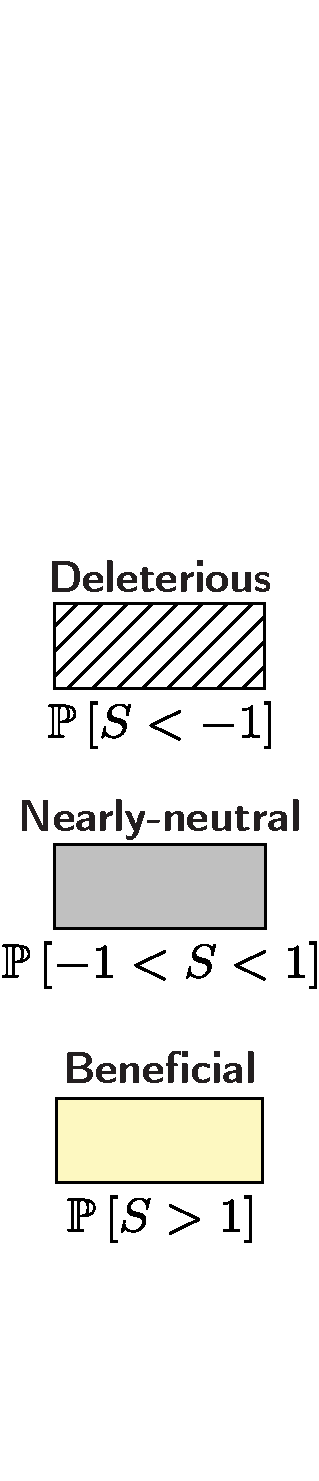
\includegraphics[width=\linewidth, page=1]{artworks/legend.polycat}
        \end{minipage}
        \captionof{figure}{~}
        \begin{minipage}{0.9\linewidth}
            \includegraphics[width=0.95\linewidth, page=1]{../experiments/5bins-polyDFE-mC/results/Theta.MutSel.neg-strong.stacked.pdf} \\
        \end{minipage}
        \begin{minipage}{0.09\linewidth}
            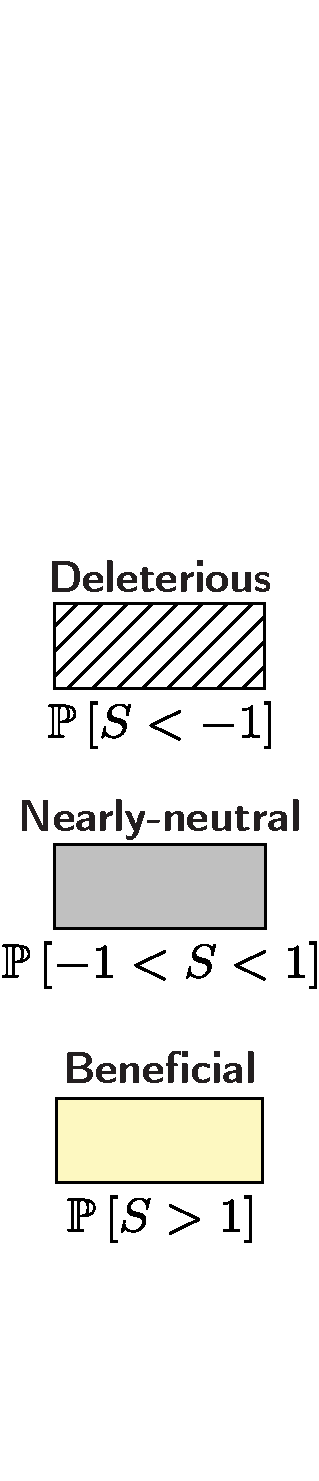
\includegraphics[width=\linewidth, page=1]{artworks/legend.polycat}
        \end{minipage}\captionof{figure}{~}
        \begin{minipage}{0.9\linewidth}
            \includegraphics[width=0.95\linewidth, page=1]{../experiments/5bins-polyDFE-mC/results/Theta.MutSel.neg.stacked.pdf} \\
        \end{minipage}
        \begin{minipage}{0.09\linewidth}
            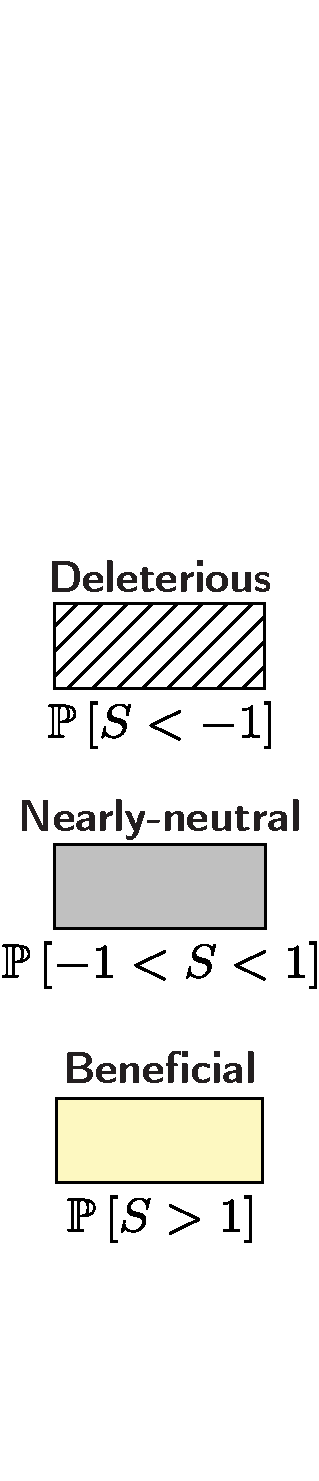
\includegraphics[width=\linewidth, page=1]{artworks/legend.polycat}
        \end{minipage}\captionof{figure}{~}
        \begin{minipage}{0.9\linewidth}
            \includegraphics[width=0.95\linewidth, page=1]{../experiments/5bins-polyDFE-mC/results/Theta.MutSel.neg-weak.stacked.pdf} \\
        \end{minipage}
        \begin{minipage}{0.09\linewidth}
            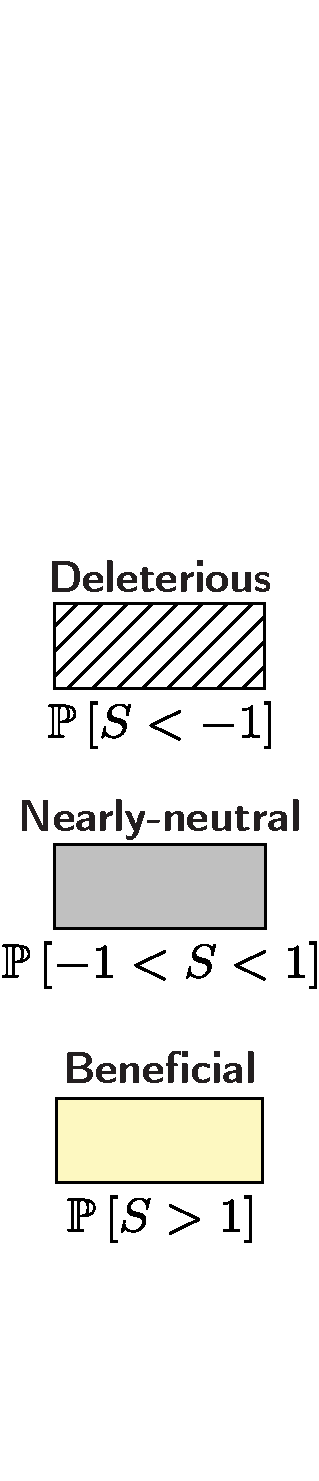
\includegraphics[width=\linewidth, page=1]{artworks/legend.polycat}
        \end{minipage}\captionof{figure}{~}
        \begin{minipage}{0.9\linewidth}
            \includegraphics[width=0.95\linewidth, page=1]{../experiments/5bins-polyDFE-mC/results/Theta.MutSel.pos-weak.stacked.pdf} \\
        \end{minipage}
        \begin{minipage}{0.09\linewidth}
            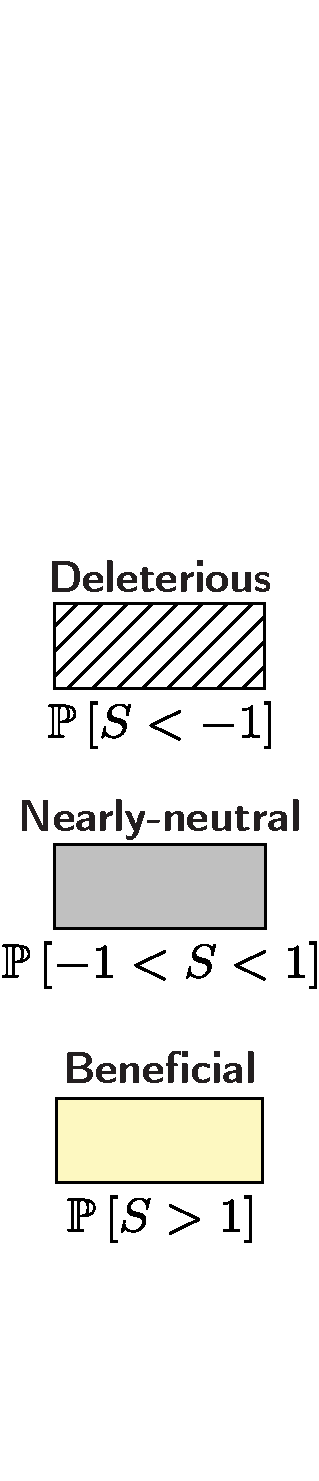
\includegraphics[width=\linewidth, page=1]{artworks/legend.polycat}
        \end{minipage}\captionof{figure}{~}
        \begin{minipage}{0.9\linewidth}
            \includegraphics[width=0.95\linewidth, page=1]{../experiments/5bins-polyDFE-mC/results/Theta.MutSel.pos.stacked.pdf}
        \end{minipage}
        \begin{minipage}{0.09\linewidth}
            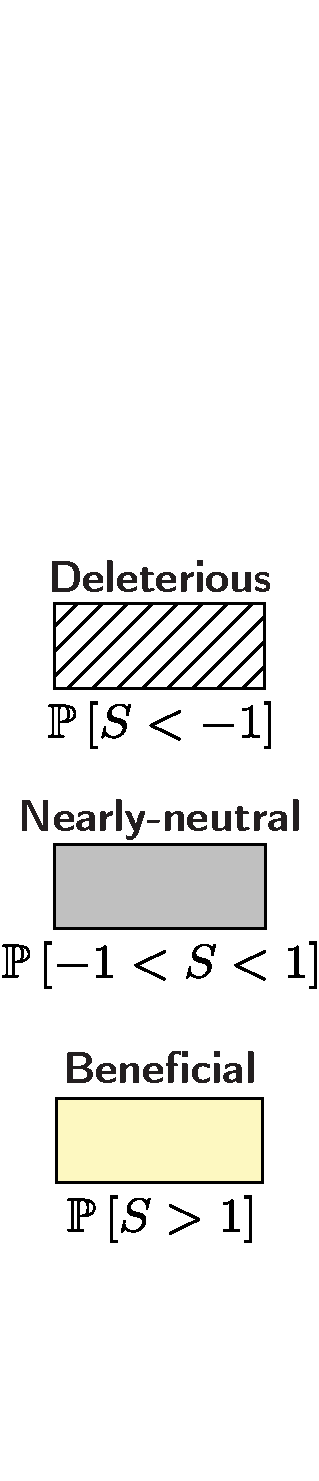
\includegraphics[width=\linewidth, page=1]{artworks/legend.polycat}
        \end{minipage}
    \end{center}
    We confirmed that higher synonymous diversity is typically accompanied by a smaller proportion of neutral mutations.
    This result is specially visible when we restricted the analysis to class of mutations that are supposedly nearly-neutral at the phylogenetic scale ($\divWeakDel$ and $\divWeakAdv$).
    This result suggests that populations with higher diversity (e.g.~\textit{Bos} or \textit{Ovis}) are more likely to discriminate whether mutations are advantageous or deleterious.
    Alternatively stated, mutations in populations with low diversity (e.g.~\textit{Homo}) are effectively nearly-neutral and behave as would a neutral mutation.
    This result is qualitatively in accordance with the nearly-neutral theory of evolution which argues that mutations are less efficiently selected for in small populations.


    \section{Mutation-selection models: histograms and SFS for each population}\label{sec:mutation-selection-models:-histograms-and-sfs-for-each-population}
    For each population, the same figure is shown.
    \begin{itemize}
        \item Top-left panel: Histogram of predicted selection coefficients ($\Sphy$) for all possible mutations away from the ancestral genome, giving the number of sites ($L$, in y-axis) across the genome with a given $\Sphy$.
        Mutations are divided into 5 classes: severely deleterious (blue), deleterious (green), weakly deleterious (light green), weakly advantageous (yellow) and advantageous (red).
        \item Top-right panel: Histogram of predicted selection coefficients ($\Sphy$) for all observed mutations in a sample of 8 individuals (out of 512 in the original dataset) of African descent.
        If they are less mutations observed than expected, this class is thus undergoing purifying selection.
        \item Bottom-left panel: The site-frequency spectrum (SFS) represents the proportion of mutations (y-axis) with a given number of derived alleles in the population (x-axis).
        SFS are drawn for a random sample of 16 alleles (mean in solid line and standard deviation in filled color) for each class of selection coefficient and for synonymous mutations which are supposedly neutral (black).
        At high frequencies, supposedly severally deleterious mutations are underrepresented.
        \item Bottom-right panel:For each class of selection (and for the set of all non-synonymous mutations), information from the SFS and the expected total mutation rate are combined at the population-genetic scale to estimate the proportion of advantageous mutations $\PpolyAdv$, of nearly-neutral mutations $\PpolyNeutral$ and of deleterious mutations $\PpolyDel$.
    \end{itemize}

    \subsection{All populations}
\begin{center}
    \includegraphics[width=0.95\linewidth, page=1]{../experiments/polyDFE-mC-non-adaptive/results/Theta.MutSel.all.stacked.pdf} \\
    \includegraphics[width=0.95\linewidth, page=1]{../experiments/polyDFE-mC-non-adaptive/results/Theta.MutSel.neg-strong.stacked.pdf} \\
    \includegraphics[width=0.95\linewidth, page=1]{../experiments/polyDFE-mC-non-adaptive/results/Theta.MutSel.neg.stacked.pdf} \\
    \includegraphics[width=0.95\linewidth, page=1]{../experiments/polyDFE-mC-non-adaptive/results/Theta.MutSel.neg-weak.stacked.pdf} \\
    \includegraphics[width=0.95\linewidth, page=1]{../experiments/polyDFE-mC-non-adaptive/results/Theta.MutSel.pos-weak.stacked.pdf} \\
    \includegraphics[width=0.95\linewidth, page=1]{../experiments/polyDFE-mC-non-adaptive/results/Theta.MutSel.pos.stacked.pdf}

\end{center}

\subsection{Bos taurus}

\subsubsection{Iran (IRBT)}

\begin{minipage}{0.49\linewidth}
    \includegraphics[width=\linewidth, page=1]{../data_processed/vcf_annotate_bins0NonAdaptive/snps.Bos_taurus.IRBT.MutSel.histogram.pdf}
\end{minipage}
\begin{minipage}{0.49\linewidth}
    \includegraphics[width=\linewidth, page=1]{../experiments/polyDFE-mC-non-adaptive/analysis/Bos_taurus.IRBT.MutSel-sfs.normalize.pdf}
\end{minipage}
\\
\begin{minipage}{0.49\linewidth}
    \includegraphics[width=\linewidth, page=1]{../data_processed/opportunities_bins0NonAdaptive/DFE.Bos_taurus.IRBT.MutSel.pdf}
\end{minipage}
\begin{minipage}{0.49\linewidth}
    \includegraphics[width=\linewidth, page=1]{../experiments/polyDFE-mC-non-adaptive/analysis/Bos_taurus.IRBT.MutSel.polyDFE_C.pdf}
\end{minipage}
\\

\subsubsection{Uganda (UGBT)}

\begin{minipage}{0.49\linewidth}
    \includegraphics[width=\linewidth, page=1]{../data_processed/vcf_annotate_bins0NonAdaptive/snps.Bos_taurus.UGBT.MutSel.histogram.pdf}
\end{minipage}
\begin{minipage}{0.49\linewidth}
    \includegraphics[width=\linewidth, page=1]{../experiments/polyDFE-mC-non-adaptive/analysis/Bos_taurus.UGBT.MutSel-sfs.normalize.pdf}
\end{minipage}
\\
\begin{minipage}{0.49\linewidth}
    \includegraphics[width=\linewidth, page=1]{../data_processed/opportunities_bins0NonAdaptive/DFE.Bos_taurus.UGBT.MutSel.pdf}
\end{minipage}
\begin{minipage}{0.49\linewidth}
    \includegraphics[width=\linewidth, page=1]{../experiments/polyDFE-mC-non-adaptive/analysis/Bos_taurus.UGBT.MutSel.polyDFE_C.pdf}
\end{minipage}
\\

\subsection{Canis familiaris}

\begin{minipage}{0.49\linewidth}
    \includegraphics[width=\linewidth, page=1]{../data_processed/vcf_annotate_bins0NonAdaptive/snps.Canis_familiaris.dogs.MutSel.histogram.pdf}
\end{minipage}
\begin{minipage}{0.49\linewidth}
    \includegraphics[width=\linewidth, page=1]{../experiments/polyDFE-mC-non-adaptive/analysis/Canis_familiaris.dogs.MutSel-sfs.normalize.pdf}
\end{minipage}
\\
\begin{minipage}{0.49\linewidth}
    \includegraphics[width=\linewidth, page=1]{../data_processed/opportunities_bins0NonAdaptive/DFE.Canis_familiaris.dogs.MutSel.pdf}
\end{minipage}
\begin{minipage}{0.49\linewidth}
    \includegraphics[width=\linewidth, page=1]{../experiments/polyDFE-mC-non-adaptive/analysis/Canis_familiaris.dogs.MutSel.polyDFE_C.pdf}
\end{minipage}
\\

\subsection{Capra}

\subsubsection{Australia (AUCH) - Capra hircus}

\begin{minipage}{0.49\linewidth}
    \includegraphics[width=\linewidth, page=1]{../data_processed/vcf_annotate_bins0NonAdaptive/snps.Capra_hircus.AUCH.MutSel.histogram.pdf}
\end{minipage}
\begin{minipage}{0.49\linewidth}
    \includegraphics[width=\linewidth, page=1]{../experiments/polyDFE-mC-non-adaptive/analysis/Capra_hircus.AUCH.MutSel-sfs.normalize.pdf}
\end{minipage}
\\
\begin{minipage}{0.49\linewidth}
    \includegraphics[width=\linewidth, page=1]{../data_processed/opportunities_bins0NonAdaptive/DFE.Capra_hircus.AUCH.MutSel.pdf}
\end{minipage}
\begin{minipage}{0.49\linewidth}
    \includegraphics[width=\linewidth, page=1]{../experiments/polyDFE-mC-non-adaptive/analysis/Capra_hircus.AUCH.MutSel.polyDFE_C.pdf}
\end{minipage}
\\

\subsubsection{France (FRCH) - Capra hircus}

\begin{minipage}{0.49\linewidth}
    \includegraphics[width=\linewidth, page=1]{../data_processed/vcf_annotate_bins0NonAdaptive/snps.Capra_hircus.FRCH.MutSel.histogram.pdf}
\end{minipage}
\begin{minipage}{0.49\linewidth}
    \includegraphics[width=\linewidth, page=1]{../experiments/polyDFE-mC-non-adaptive/analysis/Capra_hircus.FRCH.MutSel-sfs.normalize.pdf}
\end{minipage}
\\
\begin{minipage}{0.49\linewidth}
    \includegraphics[width=\linewidth, page=1]{../data_processed/opportunities_bins0NonAdaptive/DFE.Capra_hircus.FRCH.MutSel.pdf}
\end{minipage}
\begin{minipage}{0.49\linewidth}
    \includegraphics[width=\linewidth, page=1]{../experiments/polyDFE-mC-non-adaptive/analysis/Capra_hircus.FRCH.MutSel.polyDFE_C.pdf}
\end{minipage}
\\

\subsubsection{Iran (IRCA) - Capra aegagrus}

\begin{minipage}{0.49\linewidth}
    \includegraphics[width=\linewidth, page=1]{../data_processed/vcf_annotate_bins0NonAdaptive/snps.Capra_hircus.IRCA.MutSel.histogram.pdf}
\end{minipage}
\begin{minipage}{0.49\linewidth}
    \includegraphics[width=\linewidth, page=1]{../experiments/polyDFE-mC-non-adaptive/analysis/Capra_hircus.IRCA.MutSel-sfs.normalize.pdf}
\end{minipage}
\\
\begin{minipage}{0.49\linewidth}
    \includegraphics[width=\linewidth, page=1]{../data_processed/opportunities_bins0NonAdaptive/DFE.Capra_hircus.IRCA.MutSel.pdf}
\end{minipage}
\begin{minipage}{0.49\linewidth}
    \includegraphics[width=\linewidth, page=1]{../experiments/polyDFE-mC-non-adaptive/analysis/Capra_hircus.IRCA.MutSel.polyDFE_C.pdf}
\end{minipage}
\\

\subsubsection{Iran (IRCH) - Capra hircus}

\begin{minipage}{0.49\linewidth}
    \includegraphics[width=\linewidth, page=1]{../data_processed/vcf_annotate_bins0NonAdaptive/snps.Capra_hircus.IRCH.MutSel.histogram.pdf}
\end{minipage}
\begin{minipage}{0.49\linewidth}
    \includegraphics[width=\linewidth, page=1]{../experiments/polyDFE-mC-non-adaptive/analysis/Capra_hircus.IRCH.MutSel-sfs.normalize.pdf}
\end{minipage}
\\
\begin{minipage}{0.49\linewidth}
    \includegraphics[width=\linewidth, page=1]{../data_processed/opportunities_bins0NonAdaptive/DFE.Capra_hircus.IRCH.MutSel.pdf}
\end{minipage}
\begin{minipage}{0.49\linewidth}
    \includegraphics[width=\linewidth, page=1]{../experiments/polyDFE-mC-non-adaptive/analysis/Capra_hircus.IRCH.MutSel.polyDFE_C.pdf}
\end{minipage}
\\

\subsubsection{Italy (ITCH) - Capra hircus}

\begin{minipage}{0.49\linewidth}
    \includegraphics[width=\linewidth, page=1]{../data_processed/vcf_annotate_bins0NonAdaptive/snps.Capra_hircus.ITCH.MutSel.histogram.pdf}
\end{minipage}
\begin{minipage}{0.49\linewidth}
    \includegraphics[width=\linewidth, page=1]{../experiments/polyDFE-mC-non-adaptive/analysis/Capra_hircus.ITCH.MutSel-sfs.normalize.pdf}
\end{minipage}
\\
\begin{minipage}{0.49\linewidth}
    \includegraphics[width=\linewidth, page=1]{../data_processed/opportunities_bins0NonAdaptive/DFE.Capra_hircus.ITCH.MutSel.pdf}
\end{minipage}
\begin{minipage}{0.49\linewidth}
    \includegraphics[width=\linewidth, page=1]{../experiments/polyDFE-mC-non-adaptive/analysis/Capra_hircus.ITCH.MutSel.polyDFE_C.pdf}
\end{minipage}
\\

\subsubsection{Morocco (MOCH) - Capra hircus}

\begin{minipage}{0.49\linewidth}
    \includegraphics[width=\linewidth, page=1]{../data_processed/vcf_annotate_bins0NonAdaptive/snps.Capra_hircus.MOCH.MutSel.histogram.pdf}
\end{minipage}
\begin{minipage}{0.49\linewidth}
    \includegraphics[width=\linewidth, page=1]{../experiments/polyDFE-mC-non-adaptive/analysis/Capra_hircus.MOCH.MutSel-sfs.normalize.pdf}
\end{minipage}
\\
\begin{minipage}{0.49\linewidth}
    \includegraphics[width=\linewidth, page=1]{../data_processed/opportunities_bins0NonAdaptive/DFE.Capra_hircus.MOCH.MutSel.pdf}
\end{minipage}
\begin{minipage}{0.49\linewidth}
    \includegraphics[width=\linewidth, page=1]{../experiments/polyDFE-mC-non-adaptive/analysis/Capra_hircus.MOCH.MutSel.polyDFE_C.pdf}
\end{minipage}
\\

\subsection{Chlorocebus sabaeus}

\subsubsection{Barbados}

\begin{minipage}{0.49\linewidth}
    \includegraphics[width=\linewidth, page=1]{../data_processed/vcf_annotate_bins0NonAdaptive/snps.Chlorocebus_sabaeus.Barbados.MutSel.histogram.pdf}
\end{minipage}
\begin{minipage}{0.49\linewidth}
    \includegraphics[width=\linewidth, page=1]{../experiments/polyDFE-mC-non-adaptive/analysis/Chlorocebus_sabaeus.Barbados.MutSel-sfs.normalize.pdf}
\end{minipage}
\\
\begin{minipage}{0.49\linewidth}
    \includegraphics[width=\linewidth, page=1]{../data_processed/opportunities_bins0NonAdaptive/DFE.Chlorocebus_sabaeus.Barbados.MutSel.pdf}
\end{minipage}
\begin{minipage}{0.49\linewidth}
    \includegraphics[width=\linewidth, page=1]{../experiments/polyDFE-mC-non-adaptive/analysis/Chlorocebus_sabaeus.Barbados.MutSel.polyDFE_C.pdf}
\end{minipage}
\\

\subsubsection{Central African Republic (CAR)}

\begin{minipage}{0.49\linewidth}
    \includegraphics[width=\linewidth, page=1]{../data_processed/vcf_annotate_bins0NonAdaptive/snps.Chlorocebus_sabaeus.Central_African_Republic.MutSel.histogram.pdf}
\end{minipage}
\begin{minipage}{0.49\linewidth}
    \includegraphics[width=\linewidth, page=1]{../experiments/polyDFE-mC-non-adaptive/analysis/Chlorocebus_sabaeus.Central_African_Republic.MutSel-sfs.normalize.pdf}
\end{minipage}
\\
\begin{minipage}{0.49\linewidth}
    \includegraphics[width=\linewidth, page=1]{../data_processed/opportunities_bins0NonAdaptive/DFE.Chlorocebus_sabaeus.Central_African_Republic.MutSel.pdf}
\end{minipage}
\begin{minipage}{0.49\linewidth}
    \includegraphics[width=\linewidth, page=1]{../experiments/polyDFE-mC-non-adaptive/analysis/Chlorocebus_sabaeus.Central_African_Republic.MutSel.polyDFE_C.pdf}
\end{minipage}
\\

\subsubsection{Ethiopia}

\begin{minipage}{0.49\linewidth}
    \includegraphics[width=\linewidth, page=1]{../data_processed/vcf_annotate_bins0NonAdaptive/snps.Chlorocebus_sabaeus.Ethiopia.MutSel.histogram.pdf}
\end{minipage}
\begin{minipage}{0.49\linewidth}
    \includegraphics[width=\linewidth, page=1]{../experiments/polyDFE-mC-non-adaptive/analysis/Chlorocebus_sabaeus.Ethiopia.MutSel-sfs.normalize.pdf}
\end{minipage}
\\
\begin{minipage}{0.49\linewidth}
    \includegraphics[width=\linewidth, page=1]{../data_processed/opportunities_bins0NonAdaptive/DFE.Chlorocebus_sabaeus.Ethiopia.MutSel.pdf}
\end{minipage}
\begin{minipage}{0.49\linewidth}
    \includegraphics[width=\linewidth, page=1]{../experiments/polyDFE-mC-non-adaptive/analysis/Chlorocebus_sabaeus.Ethiopia.MutSel.polyDFE_C.pdf}
\end{minipage}
\\

\subsubsection{Gambia}

\begin{minipage}{0.49\linewidth}
    \includegraphics[width=\linewidth, page=1]{../data_processed/vcf_annotate_bins0NonAdaptive/snps.Chlorocebus_sabaeus.Gambia.MutSel.histogram.pdf}
\end{minipage}
\begin{minipage}{0.49\linewidth}
    \includegraphics[width=\linewidth, page=1]{../experiments/polyDFE-mC-non-adaptive/analysis/Chlorocebus_sabaeus.Gambia.MutSel-sfs.normalize.pdf}
\end{minipage}
\\
\begin{minipage}{0.49\linewidth}
    \includegraphics[width=\linewidth, page=1]{../data_processed/opportunities_bins0NonAdaptive/DFE.Chlorocebus_sabaeus.Gambia.MutSel.pdf}
\end{minipage}
\begin{minipage}{0.49\linewidth}
    \includegraphics[width=\linewidth, page=1]{../experiments/polyDFE-mC-non-adaptive/analysis/Chlorocebus_sabaeus.Gambia.MutSel.polyDFE_C.pdf}
\end{minipage}
\\

\subsubsection{Kenya}

\begin{minipage}{0.49\linewidth}
    \includegraphics[width=\linewidth, page=1]{../data_processed/vcf_annotate_bins0NonAdaptive/snps.Chlorocebus_sabaeus.Kenya.MutSel.histogram.pdf}
\end{minipage}
\begin{minipage}{0.49\linewidth}
    \includegraphics[width=\linewidth, page=1]{../experiments/polyDFE-mC-non-adaptive/analysis/Chlorocebus_sabaeus.Kenya.MutSel-sfs.normalize.pdf}
\end{minipage}
\\
\begin{minipage}{0.49\linewidth}
    \includegraphics[width=\linewidth, page=1]{../data_processed/opportunities_bins0NonAdaptive/DFE.Chlorocebus_sabaeus.Kenya.MutSel.pdf}
\end{minipage}
\begin{minipage}{0.49\linewidth}
    \includegraphics[width=\linewidth, page=1]{../experiments/polyDFE-mC-non-adaptive/analysis/Chlorocebus_sabaeus.Kenya.MutSel.polyDFE_C.pdf}
\end{minipage}
\\

\subsubsection{Nevis}

\begin{minipage}{0.49\linewidth}
    \includegraphics[width=\linewidth, page=1]{../data_processed/vcf_annotate_bins0NonAdaptive/snps.Chlorocebus_sabaeus.Nevis.MutSel.histogram.pdf}
\end{minipage}
\begin{minipage}{0.49\linewidth}
    \includegraphics[width=\linewidth, page=1]{../experiments/polyDFE-mC-non-adaptive/analysis/Chlorocebus_sabaeus.Nevis.MutSel-sfs.normalize.pdf}
\end{minipage}
\\
\begin{minipage}{0.49\linewidth}
    \includegraphics[width=\linewidth, page=1]{../data_processed/opportunities_bins0NonAdaptive/DFE.Chlorocebus_sabaeus.Nevis.MutSel.pdf}
\end{minipage}
\begin{minipage}{0.49\linewidth}
    \includegraphics[width=\linewidth, page=1]{../experiments/polyDFE-mC-non-adaptive/analysis/Chlorocebus_sabaeus.Nevis.MutSel.polyDFE_C.pdf}
\end{minipage}
\\

\subsubsection{Saint Kitts (SK)}

\begin{minipage}{0.49\linewidth}
    \includegraphics[width=\linewidth, page=1]{../data_processed/vcf_annotate_bins0NonAdaptive/snps.Chlorocebus_sabaeus.Saint_Kitts.MutSel.histogram.pdf}
\end{minipage}
\begin{minipage}{0.49\linewidth}
    \includegraphics[width=\linewidth, page=1]{../experiments/polyDFE-mC-non-adaptive/analysis/Chlorocebus_sabaeus.Saint_Kitts.MutSel-sfs.normalize.pdf}
\end{minipage}
\\
\begin{minipage}{0.49\linewidth}
    \includegraphics[width=\linewidth, page=1]{../data_processed/opportunities_bins0NonAdaptive/DFE.Chlorocebus_sabaeus.Saint_Kitts.MutSel.pdf}
\end{minipage}
\begin{minipage}{0.49\linewidth}
    \includegraphics[width=\linewidth, page=1]{../experiments/polyDFE-mC-non-adaptive/analysis/Chlorocebus_sabaeus.Saint_Kitts.MutSel.polyDFE_C.pdf}
\end{minipage}
\\

\subsubsection{South Africa (SA)}

\begin{minipage}{0.49\linewidth}
    \includegraphics[width=\linewidth, page=1]{../data_processed/vcf_annotate_bins0NonAdaptive/snps.Chlorocebus_sabaeus.South_Africa.MutSel.histogram.pdf}
\end{minipage}
\begin{minipage}{0.49\linewidth}
    \includegraphics[width=\linewidth, page=1]{../experiments/polyDFE-mC-non-adaptive/analysis/Chlorocebus_sabaeus.South_Africa.MutSel-sfs.normalize.pdf}
\end{minipage}
\\
\begin{minipage}{0.49\linewidth}
    \includegraphics[width=\linewidth, page=1]{../data_processed/opportunities_bins0NonAdaptive/DFE.Chlorocebus_sabaeus.South_Africa.MutSel.pdf}
\end{minipage}
\begin{minipage}{0.49\linewidth}
    \includegraphics[width=\linewidth, page=1]{../experiments/polyDFE-mC-non-adaptive/analysis/Chlorocebus_sabaeus.South_Africa.MutSel.polyDFE_C.pdf}
\end{minipage}
\\

\subsubsection{Zambia}

\begin{minipage}{0.49\linewidth}
    \includegraphics[width=\linewidth, page=1]{../data_processed/vcf_annotate_bins0NonAdaptive/snps.Chlorocebus_sabaeus.Zambia.MutSel.histogram.pdf}
\end{minipage}
\begin{minipage}{0.49\linewidth}
    \includegraphics[width=\linewidth, page=1]{../experiments/polyDFE-mC-non-adaptive/analysis/Chlorocebus_sabaeus.Zambia.MutSel-sfs.normalize.pdf}
\end{minipage}
\\
\begin{minipage}{0.49\linewidth}
    \includegraphics[width=\linewidth, page=1]{../data_processed/opportunities_bins0NonAdaptive/DFE.Chlorocebus_sabaeus.Zambia.MutSel.pdf}
\end{minipage}
\begin{minipage}{0.49\linewidth}
    \includegraphics[width=\linewidth, page=1]{../experiments/polyDFE-mC-non-adaptive/analysis/Chlorocebus_sabaeus.Zambia.MutSel.polyDFE_C.pdf}
\end{minipage}
\\

\subsection{Equus caballus}

\begin{minipage}{0.49\linewidth}
    \includegraphics[width=\linewidth, page=1]{../data_processed/vcf_annotate_bins0NonAdaptive/snps.Equus_caballus.up.MutSel.histogram.pdf}
\end{minipage}
\begin{minipage}{0.49\linewidth}
    \includegraphics[width=\linewidth, page=1]{../experiments/polyDFE-mC-non-adaptive/analysis/Equus_caballus.up.MutSel-sfs.normalize.pdf}
\end{minipage}
\\
\begin{minipage}{0.49\linewidth}
    \includegraphics[width=\linewidth, page=1]{../data_processed/opportunities_bins0NonAdaptive/DFE.Equus_caballus.up.MutSel.pdf}
\end{minipage}
\begin{minipage}{0.49\linewidth}
    \includegraphics[width=\linewidth, page=1]{../experiments/polyDFE-mC-non-adaptive/analysis/Equus_caballus.up.MutSel.polyDFE_C.pdf}
\end{minipage}
\\

\subsection{Homo sapiens}

\subsubsection{African (AFR)}

\begin{minipage}{0.49\linewidth}
    \includegraphics[width=\linewidth, page=1]{../data_processed/vcf_annotate_bins0NonAdaptive/snps.Homo_sapiens.AFR.MutSel.histogram.pdf}
\end{minipage}
\begin{minipage}{0.49\linewidth}
    \includegraphics[width=\linewidth, page=1]{../experiments/polyDFE-mC-non-adaptive/analysis/Homo_sapiens.AFR.MutSel-sfs.normalize.pdf}
\end{minipage}
\\
\begin{minipage}{0.49\linewidth}
    \includegraphics[width=\linewidth, page=1]{../data_processed/opportunities_bins0NonAdaptive/DFE.Homo_sapiens.AFR.MutSel.pdf}
\end{minipage}
\begin{minipage}{0.49\linewidth}
    \includegraphics[width=\linewidth, page=1]{../experiments/polyDFE-mC-non-adaptive/analysis/Homo_sapiens.AFR.MutSel.polyDFE_C.pdf}
\end{minipage}
\\

\subsubsection{Ad Mixed American (AMR)}

\begin{minipage}{0.49\linewidth}
    \includegraphics[width=\linewidth, page=1]{../data_processed/vcf_annotate_bins0NonAdaptive/snps.Homo_sapiens.AMR.MutSel.histogram.pdf}
\end{minipage}
\begin{minipage}{0.49\linewidth}
    \includegraphics[width=\linewidth, page=1]{../experiments/polyDFE-mC-non-adaptive/analysis/Homo_sapiens.AMR.MutSel-sfs.normalize.pdf}
\end{minipage}
\\
\begin{minipage}{0.49\linewidth}
    \includegraphics[width=\linewidth, page=1]{../data_processed/opportunities_bins0NonAdaptive/DFE.Homo_sapiens.AMR.MutSel.pdf}
\end{minipage}
\begin{minipage}{0.49\linewidth}
    \includegraphics[width=\linewidth, page=1]{../experiments/polyDFE-mC-non-adaptive/analysis/Homo_sapiens.AMR.MutSel.polyDFE_C.pdf}
\end{minipage}
\\

\subsubsection{East Asian (EAS)}

\begin{minipage}{0.49\linewidth}
    \includegraphics[width=\linewidth, page=1]{../data_processed/vcf_annotate_bins0NonAdaptive/snps.Homo_sapiens.EAS.MutSel.histogram.pdf}
\end{minipage}
\begin{minipage}{0.49\linewidth}
    \includegraphics[width=\linewidth, page=1]{../experiments/polyDFE-mC-non-adaptive/analysis/Homo_sapiens.EAS.MutSel-sfs.normalize.pdf}
\end{minipage}
\\
\begin{minipage}{0.49\linewidth}
    \includegraphics[width=\linewidth, page=1]{../data_processed/opportunities_bins0NonAdaptive/DFE.Homo_sapiens.EAS.MutSel.pdf}
\end{minipage}
\begin{minipage}{0.49\linewidth}
    \includegraphics[width=\linewidth, page=1]{../experiments/polyDFE-mC-non-adaptive/analysis/Homo_sapiens.EAS.MutSel.polyDFE_C.pdf}
\end{minipage}
\\

\subsubsection{European (EUR)}

\begin{minipage}{0.49\linewidth}
    \includegraphics[width=\linewidth, page=1]{../data_processed/vcf_annotate_bins0NonAdaptive/snps.Homo_sapiens.EUR.MutSel.histogram.pdf}
\end{minipage}
\begin{minipage}{0.49\linewidth}
    \includegraphics[width=\linewidth, page=1]{../experiments/polyDFE-mC-non-adaptive/analysis/Homo_sapiens.EUR.MutSel-sfs.normalize.pdf}
\end{minipage}
\\
\begin{minipage}{0.49\linewidth}
    \includegraphics[width=\linewidth, page=1]{../data_processed/opportunities_bins0NonAdaptive/DFE.Homo_sapiens.EUR.MutSel.pdf}
\end{minipage}
\begin{minipage}{0.49\linewidth}
    \includegraphics[width=\linewidth, page=1]{../experiments/polyDFE-mC-non-adaptive/analysis/Homo_sapiens.EUR.MutSel.polyDFE_C.pdf}
\end{minipage}
\\

\subsubsection{South Asian (SAS)}

\begin{minipage}{0.49\linewidth}
    \includegraphics[width=\linewidth, page=1]{../data_processed/vcf_annotate_bins0NonAdaptive/snps.Homo_sapiens.SAS.MutSel.histogram.pdf}
\end{minipage}
\begin{minipage}{0.49\linewidth}
    \includegraphics[width=\linewidth, page=1]{../experiments/polyDFE-mC-non-adaptive/analysis/Homo_sapiens.SAS.MutSel-sfs.normalize.pdf}
\end{minipage}
\\
\begin{minipage}{0.49\linewidth}
    \includegraphics[width=\linewidth, page=1]{../data_processed/opportunities_bins0NonAdaptive/DFE.Homo_sapiens.SAS.MutSel.pdf}
\end{minipage}
\begin{minipage}{0.49\linewidth}
    \includegraphics[width=\linewidth, page=1]{../experiments/polyDFE-mC-non-adaptive/analysis/Homo_sapiens.SAS.MutSel.polyDFE_C.pdf}
\end{minipage}
\\

\subsection{Ovis}

\subsubsection{Iran (IROA) - Ovis aries}

\begin{minipage}{0.49\linewidth}
    \includegraphics[width=\linewidth, page=1]{../data_processed/vcf_annotate_bins0NonAdaptive/snps.Ovis_aries.IROA.MutSel.histogram.pdf}
\end{minipage}
\begin{minipage}{0.49\linewidth}
    \includegraphics[width=\linewidth, page=1]{../experiments/polyDFE-mC-non-adaptive/analysis/Ovis_aries.IROA.MutSel-sfs.normalize.pdf}
\end{minipage}
\\
\begin{minipage}{0.49\linewidth}
    \includegraphics[width=\linewidth, page=1]{../data_processed/opportunities_bins0NonAdaptive/DFE.Ovis_aries.IROA.MutSel.pdf}
\end{minipage}
\begin{minipage}{0.49\linewidth}
    \includegraphics[width=\linewidth, page=1]{../experiments/polyDFE-mC-non-adaptive/analysis/Ovis_aries.IROA.MutSel.polyDFE_C.pdf}
\end{minipage}
\\

\subsubsection{Iran (IROO) - Ovis orientalis}

\begin{minipage}{0.49\linewidth}
    \includegraphics[width=\linewidth, page=1]{../data_processed/vcf_annotate_bins0NonAdaptive/snps.Ovis_aries.IROO.MutSel.histogram.pdf}
\end{minipage}
\begin{minipage}{0.49\linewidth}
    \includegraphics[width=\linewidth, page=1]{../experiments/polyDFE-mC-non-adaptive/analysis/Ovis_aries.IROO.MutSel-sfs.normalize.pdf}
\end{minipage}
\\
\begin{minipage}{0.49\linewidth}
    \includegraphics[width=\linewidth, page=1]{../data_processed/opportunities_bins0NonAdaptive/DFE.Ovis_aries.IROO.MutSel.pdf}
\end{minipage}
\begin{minipage}{0.49\linewidth}
    \includegraphics[width=\linewidth, page=1]{../experiments/polyDFE-mC-non-adaptive/analysis/Ovis_aries.IROO.MutSel.polyDFE_C.pdf}
\end{minipage}
\\

\subsubsection{Iran (IROV) - Ovis vignei}

\begin{minipage}{0.49\linewidth}
    \includegraphics[width=\linewidth, page=1]{../data_processed/vcf_annotate_bins0NonAdaptive/snps.Ovis_aries.IROV.MutSel.histogram.pdf}
\end{minipage}
\begin{minipage}{0.49\linewidth}
    \includegraphics[width=\linewidth, page=1]{../experiments/polyDFE-mC-non-adaptive/analysis/Ovis_aries.IROV.MutSel-sfs.normalize.pdf}
\end{minipage}
\\
\begin{minipage}{0.49\linewidth}
    \includegraphics[width=\linewidth, page=1]{../data_processed/opportunities_bins0NonAdaptive/DFE.Ovis_aries.IROV.MutSel.pdf}
\end{minipage}
\begin{minipage}{0.49\linewidth}
    \includegraphics[width=\linewidth, page=1]{../experiments/polyDFE-mC-non-adaptive/analysis/Ovis_aries.IROV.MutSel.polyDFE_C.pdf}
\end{minipage}
\\

\subsubsection{Various (ISGC) - Ovis aries}

\begin{minipage}{0.49\linewidth}
    \includegraphics[width=\linewidth, page=1]{../data_processed/vcf_annotate_bins0NonAdaptive/snps.Ovis_aries.ISGC.MutSel.histogram.pdf}
\end{minipage}
\begin{minipage}{0.49\linewidth}
    \includegraphics[width=\linewidth, page=1]{../experiments/polyDFE-mC-non-adaptive/analysis/Ovis_aries.ISGC.MutSel-sfs.normalize.pdf}
\end{minipage}
\\
\begin{minipage}{0.49\linewidth}
    \includegraphics[width=\linewidth, page=1]{../data_processed/opportunities_bins0NonAdaptive/DFE.Ovis_aries.ISGC.MutSel.pdf}
\end{minipage}
\begin{minipage}{0.49\linewidth}
    \includegraphics[width=\linewidth, page=1]{../experiments/polyDFE-mC-non-adaptive/analysis/Ovis_aries.ISGC.MutSel.polyDFE_C.pdf}
\end{minipage}
\\

\subsubsection{Morocco (MOOA) - Ovis aries}

\begin{minipage}{0.49\linewidth}
    \includegraphics[width=\linewidth, page=1]{../data_processed/vcf_annotate_bins0NonAdaptive/snps.Ovis_aries.MOOA.MutSel.histogram.pdf}
\end{minipage}
\begin{minipage}{0.49\linewidth}
    \includegraphics[width=\linewidth, page=1]{../experiments/polyDFE-mC-non-adaptive/analysis/Ovis_aries.MOOA.MutSel-sfs.normalize.pdf}
\end{minipage}
\\
\begin{minipage}{0.49\linewidth}
    \includegraphics[width=\linewidth, page=1]{../data_processed/opportunities_bins0NonAdaptive/DFE.Ovis_aries.MOOA.MutSel.pdf}
\end{minipage}
\begin{minipage}{0.49\linewidth}
    \includegraphics[width=\linewidth, page=1]{../experiments/polyDFE-mC-non-adaptive/analysis/Ovis_aries.MOOA.MutSel.polyDFE_C.pdf}
\end{minipage}
\\


    \newpage


    \section{SIFT scores}\label{sec:sift-scores}

    \subsection{Proportion of selected mutations}\label{subsec:proportion-of-selected-mutations}
    For each population, the proportion of advantageous ($\PpolyAdv$), nearly-neutral ($\PpolyNeutral$) and of deleterious ($\PpolyDel$) mutations estimated at the population-genetic scale is shown.
    Estimation is performed with SNPs with different class of SIFT scores at the phylogenetic scale.
    Population are sorted for increased synonymous diversity.

    \begin{center}
        \captionof{figure}{~}
        \begin{minipage}{0.9\linewidth}
            \includegraphics[width=0.95\linewidth, page=1]{../experiments/5bins-polyDFE-mC/results/Theta.SIFT.all.stacked.pdf}
        \end{minipage}
        \begin{minipage}{0.09\linewidth}
            \includegraphics[width=\linewidth, page=1]{artworks/legend.polycat}
        \end{minipage}
        \captionof{figure}{~}
        \begin{minipage}{0.9\linewidth}
            \includegraphics[width=0.95\linewidth, page=1]{../experiments/5bins-polyDFE-mC/results/Theta.SIFT.neg-strong.stacked.pdf} \\
        \end{minipage}
        \begin{minipage}{0.09\linewidth}
            \includegraphics[width=\linewidth, page=1]{artworks/legend.polycat}
        \end{minipage}\captionof{figure}{~}
        \begin{minipage}{0.9\linewidth}
            \includegraphics[width=0.95\linewidth, page=1]{../experiments/5bins-polyDFE-mC/results/Theta.SIFT.neg.stacked.pdf} \\
        \end{minipage}
        \begin{minipage}{0.09\linewidth}
            \includegraphics[width=\linewidth, page=1]{artworks/legend.polycat}
        \end{minipage}\captionof{figure}{~}
        \begin{minipage}{0.9\linewidth}
            \includegraphics[width=0.95\linewidth, page=1]{../experiments/5bins-polyDFE-mC/results/Theta.SIFT.neg-weak.stacked.pdf} \\
        \end{minipage}
        \begin{minipage}{0.09\linewidth}
            \includegraphics[width=\linewidth, page=1]{artworks/legend.polycat}
        \end{minipage}\captionof{figure}{~}
        \begin{minipage}{0.9\linewidth}
            \includegraphics[width=0.95\linewidth, page=1]{../experiments/5bins-polyDFE-mC/results/Theta.SIFT.pos-weak.stacked.pdf} \\
        \end{minipage}
        \begin{minipage}{0.09\linewidth}
            \includegraphics[width=\linewidth, page=1]{artworks/legend.polycat}
        \end{minipage}\captionof{figure}{~}
        \begin{minipage}{0.9\linewidth}
            \includegraphics[width=0.95\linewidth, page=1]{../experiments/5bins-polyDFE-mC/results/Theta.SIFT.pos.stacked.pdf}
        \end{minipage}
        \begin{minipage}{0.09\linewidth}
            \includegraphics[width=\linewidth, page=1]{artworks/legend.polycat}
        \end{minipage}
    \end{center}
    Sites with a higher SIFT score at the phylogenetic scale are more positively selected in the different populations.

    % The previous section showed that mutations with a higher SIFT score at the phylogenetic scale are more positively selected in the different populations.
    % However, whenever we removed the category of SNPs with the highest SIFT score ($\textrm{SIFT} \geq 0.8$), we expected the estimation of $p_+ (\textrm{SIFT} < 0.8)$ to be lower than $p_+$ (estimated on the all dataset), as we have shown that $p_+ (\Sphy < 0) < p_+$ with mutation-selection codon models.
    % Thus SIFT scores are not providing reliable information on the current selective strength exerted on mutations, at least for high SIFT scores.
    % Moreover, there is no defined threshold (here we arbitrarily used 0.8) to cut-off between advantageous and deleterious changes.


    \section{SIFT scores: histograms and SFS for each population}\label{sec:sift-scores:-histograms-and-sfs-for-each-population}
    For each population, the same figure is shown.
    \begin{itemize}
        \item Top-left panel: Histogram of SIFT score for all possible mutations away from the ancestral genome, giving the number of sites ($L$, in y-axis) across the genome with a given SIFT score.
        Mutations are divided into 5 classes: severely deleterious (blue), deleterious (green), weakly deleterious (light green), weakly advantageous (yellow) and advantageous (red).
        \item Top-right panel: Histogram of SIFT score for all observed mutations in a sample of 8 individuals (out of 512 in the original dataset) of African descent.
        If they are less mutations observed than expected, this class is thus undergoing purifying selection.
        \item Bottom-left panel: The site-frequency spectrum (SFS) represents the proportion of mutations (y-axis) with a given number of derived alleles in the population (x-axis).
        SFS are drawn for a random sample of 16 alleles (mean in solid line and standard deviation in filled color) for each class of selection coefficient and for synonymous mutations which are supposedly neutral (black).
        At high frequencies, supposedly severally deleterious mutations are underrepresented.
        \item Bottom-right panel:For each class of selection (and for the set of all non-synonymous mutations), information from the SFS and the expected total mutation rate are combined at the population-genetic scale to estimate the proportion of advantageous mutations $\PpolyAdv$, of nearly-neutral mutations $\PpolyNeutral$ and of deleterious mutations $\PpolyDel$.
    \end{itemize}
    \subsection{Bos taurus}

\subsubsection{Iran}

\begin{minipage}{0.49\linewidth}
    \includegraphics[width=\linewidth, page=1]{../data_processed/opportunities_bins5/DFE.Bos_taurus.IRBT.SIFT.pdf}
\end{minipage}
\begin{minipage}{0.49\linewidth}
    \includegraphics[width=\linewidth, page=1]{../data_processed/vcf_annotate_bins5/snps.Bos_taurus.IRBT.SIFT.histogram.pdf}
\end{minipage}
\\
\begin{minipage}{0.49\linewidth}
    \includegraphics[width=\linewidth, page=1]{../experiments/5bins-all/analysis/Bos_taurus.IRBT.SIFT-sfs.normalize.pdf}
\end{minipage}
\begin{minipage}{0.4\linewidth}
    \includegraphics[width=\linewidth, page=1]{../experiments/5bins-all/analysis/Bos_taurus.IRBT.SIFT.polyDFE_C.pdf}
\end{minipage}
\begin{minipage}{0.09\linewidth}
    \includegraphics[width=\linewidth, page=1]{artworks/legend.polycat.top}
\end{minipage}
\\

\subsubsection{Uganda}

\begin{minipage}{0.49\linewidth}
    \includegraphics[width=\linewidth, page=1]{../data_processed/opportunities_bins5/DFE.Bos_taurus.UGBT.SIFT.pdf}
\end{minipage}
\begin{minipage}{0.49\linewidth}
    \includegraphics[width=\linewidth, page=1]{../data_processed/vcf_annotate_bins5/snps.Bos_taurus.UGBT.SIFT.histogram.pdf}
\end{minipage}
\\
\begin{minipage}{0.49\linewidth}
    \includegraphics[width=\linewidth, page=1]{../experiments/5bins-all/analysis/Bos_taurus.UGBT.SIFT-sfs.normalize.pdf}
\end{minipage}
\begin{minipage}{0.4\linewidth}
    \includegraphics[width=\linewidth, page=1]{../experiments/5bins-all/analysis/Bos_taurus.UGBT.SIFT.polyDFE_C.pdf}
\end{minipage}
\begin{minipage}{0.09\linewidth}
    \includegraphics[width=\linewidth, page=1]{artworks/legend.polycat.top}
\end{minipage}
\\

\subsection{Capra}

\subsubsection{Australia}

\begin{minipage}{0.49\linewidth}
    \includegraphics[width=\linewidth, page=1]{../data_processed/opportunities_bins5/DFE.Capra_hircus.AUCH.SIFT.pdf}
\end{minipage}
\begin{minipage}{0.49\linewidth}
    \includegraphics[width=\linewidth, page=1]{../data_processed/vcf_annotate_bins5/snps.Capra_hircus.AUCH.SIFT.histogram.pdf}
\end{minipage}
\\
\begin{minipage}{0.49\linewidth}
    \includegraphics[width=\linewidth, page=1]{../experiments/5bins-all/analysis/Capra_hircus.AUCH.SIFT-sfs.normalize.pdf}
\end{minipage}
\begin{minipage}{0.4\linewidth}
    \includegraphics[width=\linewidth, page=1]{../experiments/5bins-all/analysis/Capra_hircus.AUCH.SIFT.polyDFE_C.pdf}
\end{minipage}
\begin{minipage}{0.09\linewidth}
    \includegraphics[width=\linewidth, page=1]{artworks/legend.polycat.top}
\end{minipage}
\\

\subsubsection{France}

\begin{minipage}{0.49\linewidth}
    \includegraphics[width=\linewidth, page=1]{../data_processed/opportunities_bins5/DFE.Capra_hircus.FRCH.SIFT.pdf}
\end{minipage}
\begin{minipage}{0.49\linewidth}
    \includegraphics[width=\linewidth, page=1]{../data_processed/vcf_annotate_bins5/snps.Capra_hircus.FRCH.SIFT.histogram.pdf}
\end{minipage}
\\
\begin{minipage}{0.49\linewidth}
    \includegraphics[width=\linewidth, page=1]{../experiments/5bins-all/analysis/Capra_hircus.FRCH.SIFT-sfs.normalize.pdf}
\end{minipage}
\begin{minipage}{0.4\linewidth}
    \includegraphics[width=\linewidth, page=1]{../experiments/5bins-all/analysis/Capra_hircus.FRCH.SIFT.polyDFE_C.pdf}
\end{minipage}
\begin{minipage}{0.09\linewidth}
    \includegraphics[width=\linewidth, page=1]{artworks/legend.polycat.top}
\end{minipage}
\\

\subsubsection{Iran (C. aegagrus)}

\begin{minipage}{0.49\linewidth}
    \includegraphics[width=\linewidth, page=1]{../data_processed/opportunities_bins5/DFE.Capra_hircus.IRCA.SIFT.pdf}
\end{minipage}
\begin{minipage}{0.49\linewidth}
    \includegraphics[width=\linewidth, page=1]{../data_processed/vcf_annotate_bins5/snps.Capra_hircus.IRCA.SIFT.histogram.pdf}
\end{minipage}
\\
\begin{minipage}{0.49\linewidth}
    \includegraphics[width=\linewidth, page=1]{../experiments/5bins-all/analysis/Capra_hircus.IRCA.SIFT-sfs.normalize.pdf}
\end{minipage}
\begin{minipage}{0.4\linewidth}
    \includegraphics[width=\linewidth, page=1]{../experiments/5bins-all/analysis/Capra_hircus.IRCA.SIFT.polyDFE_C.pdf}
\end{minipage}
\begin{minipage}{0.09\linewidth}
    \includegraphics[width=\linewidth, page=1]{artworks/legend.polycat.top}
\end{minipage}
\\

\subsubsection{Iran}

\begin{minipage}{0.49\linewidth}
    \includegraphics[width=\linewidth, page=1]{../data_processed/opportunities_bins5/DFE.Capra_hircus.IRCH.SIFT.pdf}
\end{minipage}
\begin{minipage}{0.49\linewidth}
    \includegraphics[width=\linewidth, page=1]{../data_processed/vcf_annotate_bins5/snps.Capra_hircus.IRCH.SIFT.histogram.pdf}
\end{minipage}
\\
\begin{minipage}{0.49\linewidth}
    \includegraphics[width=\linewidth, page=1]{../experiments/5bins-all/analysis/Capra_hircus.IRCH.SIFT-sfs.normalize.pdf}
\end{minipage}
\begin{minipage}{0.4\linewidth}
    \includegraphics[width=\linewidth, page=1]{../experiments/5bins-all/analysis/Capra_hircus.IRCH.SIFT.polyDFE_C.pdf}
\end{minipage}
\begin{minipage}{0.09\linewidth}
    \includegraphics[width=\linewidth, page=1]{artworks/legend.polycat.top}
\end{minipage}
\\

\subsubsection{Italy}

\begin{minipage}{0.49\linewidth}
    \includegraphics[width=\linewidth, page=1]{../data_processed/opportunities_bins5/DFE.Capra_hircus.ITCH.SIFT.pdf}
\end{minipage}
\begin{minipage}{0.49\linewidth}
    \includegraphics[width=\linewidth, page=1]{../data_processed/vcf_annotate_bins5/snps.Capra_hircus.ITCH.SIFT.histogram.pdf}
\end{minipage}
\\
\begin{minipage}{0.49\linewidth}
    \includegraphics[width=\linewidth, page=1]{../experiments/5bins-all/analysis/Capra_hircus.ITCH.SIFT-sfs.normalize.pdf}
\end{minipage}
\begin{minipage}{0.4\linewidth}
    \includegraphics[width=\linewidth, page=1]{../experiments/5bins-all/analysis/Capra_hircus.ITCH.SIFT.polyDFE_C.pdf}
\end{minipage}
\begin{minipage}{0.09\linewidth}
    \includegraphics[width=\linewidth, page=1]{artworks/legend.polycat.top}
\end{minipage}
\\

\subsubsection{Morocco}

\begin{minipage}{0.49\linewidth}
    \includegraphics[width=\linewidth, page=1]{../data_processed/opportunities_bins5/DFE.Capra_hircus.MOCH.SIFT.pdf}
\end{minipage}
\begin{minipage}{0.49\linewidth}
    \includegraphics[width=\linewidth, page=1]{../data_processed/vcf_annotate_bins5/snps.Capra_hircus.MOCH.SIFT.histogram.pdf}
\end{minipage}
\\
\begin{minipage}{0.49\linewidth}
    \includegraphics[width=\linewidth, page=1]{../experiments/5bins-all/analysis/Capra_hircus.MOCH.SIFT-sfs.normalize.pdf}
\end{minipage}
\begin{minipage}{0.4\linewidth}
    \includegraphics[width=\linewidth, page=1]{../experiments/5bins-all/analysis/Capra_hircus.MOCH.SIFT.polyDFE_C.pdf}
\end{minipage}
\begin{minipage}{0.09\linewidth}
    \includegraphics[width=\linewidth, page=1]{artworks/legend.polycat.top}
\end{minipage}
\\

\subsection{Chlorocebus sabaeus}

\subsubsection{Barbados}

\begin{minipage}{0.49\linewidth}
    \includegraphics[width=\linewidth, page=1]{../data_processed/opportunities_bins5/DFE.Chlorocebus_sabaeus.Barbados.SIFT.pdf}
\end{minipage}
\begin{minipage}{0.49\linewidth}
    \includegraphics[width=\linewidth, page=1]{../data_processed/vcf_annotate_bins5/snps.Chlorocebus_sabaeus.Barbados.SIFT.histogram.pdf}
\end{minipage}
\\
\begin{minipage}{0.49\linewidth}
    \includegraphics[width=\linewidth, page=1]{../experiments/5bins-all/analysis/Chlorocebus_sabaeus.Barbados.SIFT-sfs.normalize.pdf}
\end{minipage}
\begin{minipage}{0.4\linewidth}
    \includegraphics[width=\linewidth, page=1]{../experiments/5bins-all/analysis/Chlorocebus_sabaeus.Barbados.SIFT.polyDFE_C.pdf}
\end{minipage}
\begin{minipage}{0.09\linewidth}
    \includegraphics[width=\linewidth, page=1]{artworks/legend.polycat.top}
\end{minipage}
\\

\subsubsection{Central Afr. Rep.}

\begin{minipage}{0.49\linewidth}
    \includegraphics[width=\linewidth, page=1]{../data_processed/opportunities_bins5/DFE.Chlorocebus_sabaeus.Central_African_Republic.SIFT.pdf}
\end{minipage}
\begin{minipage}{0.49\linewidth}
    \includegraphics[width=\linewidth, page=1]{../data_processed/vcf_annotate_bins5/snps.Chlorocebus_sabaeus.Central_African_Republic.SIFT.histogram.pdf}
\end{minipage}
\\
\begin{minipage}{0.49\linewidth}
    \includegraphics[width=\linewidth, page=1]{../experiments/5bins-all/analysis/Chlorocebus_sabaeus.Central_African_Republic.SIFT-sfs.normalize.pdf}
\end{minipage}
\begin{minipage}{0.4\linewidth}
    \includegraphics[width=\linewidth, page=1]{../experiments/5bins-all/analysis/Chlorocebus_sabaeus.Central_African_Republic.SIFT.polyDFE_C.pdf}
\end{minipage}
\begin{minipage}{0.09\linewidth}
    \includegraphics[width=\linewidth, page=1]{artworks/legend.polycat.top}
\end{minipage}
\\

\subsubsection{Ethiopia}

\begin{minipage}{0.49\linewidth}
    \includegraphics[width=\linewidth, page=1]{../data_processed/opportunities_bins5/DFE.Chlorocebus_sabaeus.Ethiopia.SIFT.pdf}
\end{minipage}
\begin{minipage}{0.49\linewidth}
    \includegraphics[width=\linewidth, page=1]{../data_processed/vcf_annotate_bins5/snps.Chlorocebus_sabaeus.Ethiopia.SIFT.histogram.pdf}
\end{minipage}
\\
\begin{minipage}{0.49\linewidth}
    \includegraphics[width=\linewidth, page=1]{../experiments/5bins-all/analysis/Chlorocebus_sabaeus.Ethiopia.SIFT-sfs.normalize.pdf}
\end{minipage}
\begin{minipage}{0.4\linewidth}
    \includegraphics[width=\linewidth, page=1]{../experiments/5bins-all/analysis/Chlorocebus_sabaeus.Ethiopia.SIFT.polyDFE_C.pdf}
\end{minipage}
\begin{minipage}{0.09\linewidth}
    \includegraphics[width=\linewidth, page=1]{artworks/legend.polycat.top}
\end{minipage}
\\

\subsubsection{Gambia}

\begin{minipage}{0.49\linewidth}
    \includegraphics[width=\linewidth, page=1]{../data_processed/opportunities_bins5/DFE.Chlorocebus_sabaeus.Gambia.SIFT.pdf}
\end{minipage}
\begin{minipage}{0.49\linewidth}
    \includegraphics[width=\linewidth, page=1]{../data_processed/vcf_annotate_bins5/snps.Chlorocebus_sabaeus.Gambia.SIFT.histogram.pdf}
\end{minipage}
\\
\begin{minipage}{0.49\linewidth}
    \includegraphics[width=\linewidth, page=1]{../experiments/5bins-all/analysis/Chlorocebus_sabaeus.Gambia.SIFT-sfs.normalize.pdf}
\end{minipage}
\begin{minipage}{0.4\linewidth}
    \includegraphics[width=\linewidth, page=1]{../experiments/5bins-all/analysis/Chlorocebus_sabaeus.Gambia.SIFT.polyDFE_C.pdf}
\end{minipage}
\begin{minipage}{0.09\linewidth}
    \includegraphics[width=\linewidth, page=1]{artworks/legend.polycat.top}
\end{minipage}
\\

\subsubsection{Kenya}

\begin{minipage}{0.49\linewidth}
    \includegraphics[width=\linewidth, page=1]{../data_processed/opportunities_bins5/DFE.Chlorocebus_sabaeus.Kenya.SIFT.pdf}
\end{minipage}
\begin{minipage}{0.49\linewidth}
    \includegraphics[width=\linewidth, page=1]{../data_processed/vcf_annotate_bins5/snps.Chlorocebus_sabaeus.Kenya.SIFT.histogram.pdf}
\end{minipage}
\\
\begin{minipage}{0.49\linewidth}
    \includegraphics[width=\linewidth, page=1]{../experiments/5bins-all/analysis/Chlorocebus_sabaeus.Kenya.SIFT-sfs.normalize.pdf}
\end{minipage}
\begin{minipage}{0.4\linewidth}
    \includegraphics[width=\linewidth, page=1]{../experiments/5bins-all/analysis/Chlorocebus_sabaeus.Kenya.SIFT.polyDFE_C.pdf}
\end{minipage}
\begin{minipage}{0.09\linewidth}
    \includegraphics[width=\linewidth, page=1]{artworks/legend.polycat.top}
\end{minipage}
\\

\subsubsection{Nevis}

\begin{minipage}{0.49\linewidth}
    \includegraphics[width=\linewidth, page=1]{../data_processed/opportunities_bins5/DFE.Chlorocebus_sabaeus.Nevis.SIFT.pdf}
\end{minipage}
\begin{minipage}{0.49\linewidth}
    \includegraphics[width=\linewidth, page=1]{../data_processed/vcf_annotate_bins5/snps.Chlorocebus_sabaeus.Nevis.SIFT.histogram.pdf}
\end{minipage}
\\
\begin{minipage}{0.49\linewidth}
    \includegraphics[width=\linewidth, page=1]{../experiments/5bins-all/analysis/Chlorocebus_sabaeus.Nevis.SIFT-sfs.normalize.pdf}
\end{minipage}
\begin{minipage}{0.4\linewidth}
    \includegraphics[width=\linewidth, page=1]{../experiments/5bins-all/analysis/Chlorocebus_sabaeus.Nevis.SIFT.polyDFE_C.pdf}
\end{minipage}
\begin{minipage}{0.09\linewidth}
    \includegraphics[width=\linewidth, page=1]{artworks/legend.polycat.top}
\end{minipage}
\\

\subsubsection{Saint Kitts}

\begin{minipage}{0.49\linewidth}
    \includegraphics[width=\linewidth, page=1]{../data_processed/opportunities_bins5/DFE.Chlorocebus_sabaeus.Saint_Kitts.SIFT.pdf}
\end{minipage}
\begin{minipage}{0.49\linewidth}
    \includegraphics[width=\linewidth, page=1]{../data_processed/vcf_annotate_bins5/snps.Chlorocebus_sabaeus.Saint_Kitts.SIFT.histogram.pdf}
\end{minipage}
\\
\begin{minipage}{0.49\linewidth}
    \includegraphics[width=\linewidth, page=1]{../experiments/5bins-all/analysis/Chlorocebus_sabaeus.Saint_Kitts.SIFT-sfs.normalize.pdf}
\end{minipage}
\begin{minipage}{0.4\linewidth}
    \includegraphics[width=\linewidth, page=1]{../experiments/5bins-all/analysis/Chlorocebus_sabaeus.Saint_Kitts.SIFT.polyDFE_C.pdf}
\end{minipage}
\begin{minipage}{0.09\linewidth}
    \includegraphics[width=\linewidth, page=1]{artworks/legend.polycat.top}
\end{minipage}
\\

\subsubsection{South Africa}

\begin{minipage}{0.49\linewidth}
    \includegraphics[width=\linewidth, page=1]{../data_processed/opportunities_bins5/DFE.Chlorocebus_sabaeus.South_Africa.SIFT.pdf}
\end{minipage}
\begin{minipage}{0.49\linewidth}
    \includegraphics[width=\linewidth, page=1]{../data_processed/vcf_annotate_bins5/snps.Chlorocebus_sabaeus.South_Africa.SIFT.histogram.pdf}
\end{minipage}
\\
\begin{minipage}{0.49\linewidth}
    \includegraphics[width=\linewidth, page=1]{../experiments/5bins-all/analysis/Chlorocebus_sabaeus.South_Africa.SIFT-sfs.normalize.pdf}
\end{minipage}
\begin{minipage}{0.4\linewidth}
    \includegraphics[width=\linewidth, page=1]{../experiments/5bins-all/analysis/Chlorocebus_sabaeus.South_Africa.SIFT.polyDFE_C.pdf}
\end{minipage}
\begin{minipage}{0.09\linewidth}
    \includegraphics[width=\linewidth, page=1]{artworks/legend.polycat.top}
\end{minipage}
\\

\subsubsection{Zambia}

\begin{minipage}{0.49\linewidth}
    \includegraphics[width=\linewidth, page=1]{../data_processed/opportunities_bins5/DFE.Chlorocebus_sabaeus.Zambia.SIFT.pdf}
\end{minipage}
\begin{minipage}{0.49\linewidth}
    \includegraphics[width=\linewidth, page=1]{../data_processed/vcf_annotate_bins5/snps.Chlorocebus_sabaeus.Zambia.SIFT.histogram.pdf}
\end{minipage}
\\
\begin{minipage}{0.49\linewidth}
    \includegraphics[width=\linewidth, page=1]{../experiments/5bins-all/analysis/Chlorocebus_sabaeus.Zambia.SIFT-sfs.normalize.pdf}
\end{minipage}
\begin{minipage}{0.4\linewidth}
    \includegraphics[width=\linewidth, page=1]{../experiments/5bins-all/analysis/Chlorocebus_sabaeus.Zambia.SIFT.polyDFE_C.pdf}
\end{minipage}
\begin{minipage}{0.09\linewidth}
    \includegraphics[width=\linewidth, page=1]{artworks/legend.polycat.top}
\end{minipage}
\\

\subsection{Equus caballus}

\begin{minipage}{0.49\linewidth}
    \includegraphics[width=\linewidth, page=1]{../data_processed/opportunities_bins5/DFE.Equus_caballus.up.SIFT.pdf}
\end{minipage}
\begin{minipage}{0.49\linewidth}
    \includegraphics[width=\linewidth, page=1]{../data_processed/vcf_annotate_bins5/snps.Equus_caballus.up.SIFT.histogram.pdf}
\end{minipage}
\\
\begin{minipage}{0.49\linewidth}
    \includegraphics[width=\linewidth, page=1]{../experiments/5bins-all/analysis/Equus_caballus.up.SIFT-sfs.normalize.pdf}
\end{minipage}
\begin{minipage}{0.4\linewidth}
    \includegraphics[width=\linewidth, page=1]{../experiments/5bins-all/analysis/Equus_caballus.up.SIFT.polyDFE_C.pdf}
\end{minipage}
\begin{minipage}{0.09\linewidth}
    \includegraphics[width=\linewidth, page=1]{artworks/legend.polycat.top}
\end{minipage}
\\

\subsection{Homo sapiens}

\subsubsection{African}

\begin{minipage}{0.49\linewidth}
    \includegraphics[width=\linewidth, page=1]{../data_processed/opportunities_bins5/DFE.Homo_sapiens.AFR.SIFT.pdf}
\end{minipage}
\begin{minipage}{0.49\linewidth}
    \includegraphics[width=\linewidth, page=1]{../data_processed/vcf_annotate_bins5/snps.Homo_sapiens.AFR.SIFT.histogram.pdf}
\end{minipage}
\\
\begin{minipage}{0.49\linewidth}
    \includegraphics[width=\linewidth, page=1]{../experiments/5bins-all/analysis/Homo_sapiens.AFR.SIFT-sfs.normalize.pdf}
\end{minipage}
\begin{minipage}{0.4\linewidth}
    \includegraphics[width=\linewidth, page=1]{../experiments/5bins-all/analysis/Homo_sapiens.AFR.SIFT.polyDFE_C.pdf}
\end{minipage}
\begin{minipage}{0.09\linewidth}
    \includegraphics[width=\linewidth, page=1]{artworks/legend.polycat.top}
\end{minipage}
\\

\subsubsection{Admixed American}

\begin{minipage}{0.49\linewidth}
    \includegraphics[width=\linewidth, page=1]{../data_processed/opportunities_bins5/DFE.Homo_sapiens.AMR.SIFT.pdf}
\end{minipage}
\begin{minipage}{0.49\linewidth}
    \includegraphics[width=\linewidth, page=1]{../data_processed/vcf_annotate_bins5/snps.Homo_sapiens.AMR.SIFT.histogram.pdf}
\end{minipage}
\\
\begin{minipage}{0.49\linewidth}
    \includegraphics[width=\linewidth, page=1]{../experiments/5bins-all/analysis/Homo_sapiens.AMR.SIFT-sfs.normalize.pdf}
\end{minipage}
\begin{minipage}{0.4\linewidth}
    \includegraphics[width=\linewidth, page=1]{../experiments/5bins-all/analysis/Homo_sapiens.AMR.SIFT.polyDFE_C.pdf}
\end{minipage}
\begin{minipage}{0.09\linewidth}
    \includegraphics[width=\linewidth, page=1]{artworks/legend.polycat.top}
\end{minipage}
\\

\subsubsection{East Asian}

\begin{minipage}{0.49\linewidth}
    \includegraphics[width=\linewidth, page=1]{../data_processed/opportunities_bins5/DFE.Homo_sapiens.EAS.SIFT.pdf}
\end{minipage}
\begin{minipage}{0.49\linewidth}
    \includegraphics[width=\linewidth, page=1]{../data_processed/vcf_annotate_bins5/snps.Homo_sapiens.EAS.SIFT.histogram.pdf}
\end{minipage}
\\
\begin{minipage}{0.49\linewidth}
    \includegraphics[width=\linewidth, page=1]{../experiments/5bins-all/analysis/Homo_sapiens.EAS.SIFT-sfs.normalize.pdf}
\end{minipage}
\begin{minipage}{0.4\linewidth}
    \includegraphics[width=\linewidth, page=1]{../experiments/5bins-all/analysis/Homo_sapiens.EAS.SIFT.polyDFE_C.pdf}
\end{minipage}
\begin{minipage}{0.09\linewidth}
    \includegraphics[width=\linewidth, page=1]{artworks/legend.polycat.top}
\end{minipage}
\\

\subsubsection{European}

\begin{minipage}{0.49\linewidth}
    \includegraphics[width=\linewidth, page=1]{../data_processed/opportunities_bins5/DFE.Homo_sapiens.EUR.SIFT.pdf}
\end{minipage}
\begin{minipage}{0.49\linewidth}
    \includegraphics[width=\linewidth, page=1]{../data_processed/vcf_annotate_bins5/snps.Homo_sapiens.EUR.SIFT.histogram.pdf}
\end{minipage}
\\
\begin{minipage}{0.49\linewidth}
    \includegraphics[width=\linewidth, page=1]{../experiments/5bins-all/analysis/Homo_sapiens.EUR.SIFT-sfs.normalize.pdf}
\end{minipage}
\begin{minipage}{0.4\linewidth}
    \includegraphics[width=\linewidth, page=1]{../experiments/5bins-all/analysis/Homo_sapiens.EUR.SIFT.polyDFE_C.pdf}
\end{minipage}
\begin{minipage}{0.09\linewidth}
    \includegraphics[width=\linewidth, page=1]{artworks/legend.polycat.top}
\end{minipage}
\\

\subsubsection{South Asian}

\begin{minipage}{0.49\linewidth}
    \includegraphics[width=\linewidth, page=1]{../data_processed/opportunities_bins5/DFE.Homo_sapiens.SAS.SIFT.pdf}
\end{minipage}
\begin{minipage}{0.49\linewidth}
    \includegraphics[width=\linewidth, page=1]{../data_processed/vcf_annotate_bins5/snps.Homo_sapiens.SAS.SIFT.histogram.pdf}
\end{minipage}
\\
\begin{minipage}{0.49\linewidth}
    \includegraphics[width=\linewidth, page=1]{../experiments/5bins-all/analysis/Homo_sapiens.SAS.SIFT-sfs.normalize.pdf}
\end{minipage}
\begin{minipage}{0.4\linewidth}
    \includegraphics[width=\linewidth, page=1]{../experiments/5bins-all/analysis/Homo_sapiens.SAS.SIFT.polyDFE_C.pdf}
\end{minipage}
\begin{minipage}{0.09\linewidth}
    \includegraphics[width=\linewidth, page=1]{artworks/legend.polycat.top}
\end{minipage}
\\

\subsection{Ovis}

\subsubsection{Iran}

\begin{minipage}{0.49\linewidth}
    \includegraphics[width=\linewidth, page=1]{../data_processed/opportunities_bins5/DFE.Ovis_aries.IROA.SIFT.pdf}
\end{minipage}
\begin{minipage}{0.49\linewidth}
    \includegraphics[width=\linewidth, page=1]{../data_processed/vcf_annotate_bins5/snps.Ovis_aries.IROA.SIFT.histogram.pdf}
\end{minipage}
\\
\begin{minipage}{0.49\linewidth}
    \includegraphics[width=\linewidth, page=1]{../experiments/5bins-all/analysis/Ovis_aries.IROA.SIFT-sfs.normalize.pdf}
\end{minipage}
\begin{minipage}{0.4\linewidth}
    \includegraphics[width=\linewidth, page=1]{../experiments/5bins-all/analysis/Ovis_aries.IROA.SIFT.polyDFE_C.pdf}
\end{minipage}
\begin{minipage}{0.09\linewidth}
    \includegraphics[width=\linewidth, page=1]{artworks/legend.polycat.top}
\end{minipage}
\\

\subsubsection{Iran (O. orientalis)}

\begin{minipage}{0.49\linewidth}
    \includegraphics[width=\linewidth, page=1]{../data_processed/opportunities_bins5/DFE.Ovis_aries.IROO.SIFT.pdf}
\end{minipage}
\begin{minipage}{0.49\linewidth}
    \includegraphics[width=\linewidth, page=1]{../data_processed/vcf_annotate_bins5/snps.Ovis_aries.IROO.SIFT.histogram.pdf}
\end{minipage}
\\
\begin{minipage}{0.49\linewidth}
    \includegraphics[width=\linewidth, page=1]{../experiments/5bins-all/analysis/Ovis_aries.IROO.SIFT-sfs.normalize.pdf}
\end{minipage}
\begin{minipage}{0.4\linewidth}
    \includegraphics[width=\linewidth, page=1]{../experiments/5bins-all/analysis/Ovis_aries.IROO.SIFT.polyDFE_C.pdf}
\end{minipage}
\begin{minipage}{0.09\linewidth}
    \includegraphics[width=\linewidth, page=1]{artworks/legend.polycat.top}
\end{minipage}
\\

\subsubsection{Iran (O. vignei)}

\begin{minipage}{0.49\linewidth}
    \includegraphics[width=\linewidth, page=1]{../data_processed/opportunities_bins5/DFE.Ovis_aries.IROV.SIFT.pdf}
\end{minipage}
\begin{minipage}{0.49\linewidth}
    \includegraphics[width=\linewidth, page=1]{../data_processed/vcf_annotate_bins5/snps.Ovis_aries.IROV.SIFT.histogram.pdf}
\end{minipage}
\\
\begin{minipage}{0.49\linewidth}
    \includegraphics[width=\linewidth, page=1]{../experiments/5bins-all/analysis/Ovis_aries.IROV.SIFT-sfs.normalize.pdf}
\end{minipage}
\begin{minipage}{0.4\linewidth}
    \includegraphics[width=\linewidth, page=1]{../experiments/5bins-all/analysis/Ovis_aries.IROV.SIFT.polyDFE_C.pdf}
\end{minipage}
\begin{minipage}{0.09\linewidth}
    \includegraphics[width=\linewidth, page=1]{artworks/legend.polycat.top}
\end{minipage}
\\

\subsubsection{Various}

\begin{minipage}{0.49\linewidth}
    \includegraphics[width=\linewidth, page=1]{../data_processed/opportunities_bins5/DFE.Ovis_aries.ISGC.SIFT.pdf}
\end{minipage}
\begin{minipage}{0.49\linewidth}
    \includegraphics[width=\linewidth, page=1]{../data_processed/vcf_annotate_bins5/snps.Ovis_aries.ISGC.SIFT.histogram.pdf}
\end{minipage}
\\
\begin{minipage}{0.49\linewidth}
    \includegraphics[width=\linewidth, page=1]{../experiments/5bins-all/analysis/Ovis_aries.ISGC.SIFT-sfs.normalize.pdf}
\end{minipage}
\begin{minipage}{0.4\linewidth}
    \includegraphics[width=\linewidth, page=1]{../experiments/5bins-all/analysis/Ovis_aries.ISGC.SIFT.polyDFE_C.pdf}
\end{minipage}
\begin{minipage}{0.09\linewidth}
    \includegraphics[width=\linewidth, page=1]{artworks/legend.polycat.top}
\end{minipage}
\\

\subsubsection{Morocco}

\begin{minipage}{0.49\linewidth}
    \includegraphics[width=\linewidth, page=1]{../data_processed/opportunities_bins5/DFE.Ovis_aries.MOOA.SIFT.pdf}
\end{minipage}
\begin{minipage}{0.49\linewidth}
    \includegraphics[width=\linewidth, page=1]{../data_processed/vcf_annotate_bins5/snps.Ovis_aries.MOOA.SIFT.histogram.pdf}
\end{minipage}
\\
\begin{minipage}{0.49\linewidth}
    \includegraphics[width=\linewidth, page=1]{../experiments/5bins-all/analysis/Ovis_aries.MOOA.SIFT-sfs.normalize.pdf}
\end{minipage}
\begin{minipage}{0.49\linewidth}
    \includegraphics[width=\linewidth, page=1]{../experiments/5bins-all/analysis/Ovis_aries.MOOA.SIFT.polyDFE_C.pdf}
\end{minipage}
\\ 


\end{document}